\documentclass[11pt]{article}

\usepackage[margin=1in]{geometry}
\usepackage{graphicx}
\usepackage{booktabs}
\usepackage{amsmath}
\usepackage{amssymb}
\usepackage{caption}
\usepackage{float}
\usepackage{xcolor}
\usepackage[hidelinks]{hyperref}

\graphicspath{{figs/}{../../logs/}}
\captionsetup{font=small, labelfont=bf}

\newcommand{\code}[1]{\texttt{#1}}

\title{Power-Share Setpoint Sweep under Trapezoidal Load:\\
Bench Results, a Minority-Channel Dropout Limit Cycle,\\
and Validation of Its Firmware Mitigation}
\author{Ricky Tan\\ \small\texttt{rstan@ucdavis.edu}}
\date{2026-08-11 (revised 2026-08-13 with the firmware~v3, v4, v5, and~v6
validation sweeps)}

\begin{document}
\maketitle

\begin{abstract}
Seven bench runs (\code{TP0007}--\code{TP0013}) sweep the power-share setpoint of the
DC balancer board's droop-based share controller across the full $[0,1]$ range under an
identical trapezoidal motor-current profile. Steady-state tracking is excellent and
unbiased at every setpoint (hold-window mean error $<10^{-3}$ across the sweep), and
interior setpoints settle in under 2\,s with no actuator saturation. Two runs, however,
expose a previously unobserved failure mode: at asymmetric setpoints (0.30 and 0.85)
and low total current ($\lesssim 1.2$\,A), the loop enters a sustained
17--18.5\,Hz \emph{minority-channel dropout limit cycle}. In its severe form
(\code{TP0010}, setpoint 0.30) the two boost channels conduct mutually exclusively,
reconnect spikes reach 3.6\,A, and the bus collapses below 15\,V sixty-four times ---
to a minimum of 6.55\,V on a 15.9\,V rail --- without raising any fault. This paper
documents the sweep, characterizes the limit cycle, evaluates candidate mechanisms,
and recommends firmware and test-procedure changes. The event is logged as a
nondestructive datapoint in the board's bring-up failure record.

A second campaign (Section~\ref{sec:validation}; \code{TP0014}--\code{TP0038},
\code{WP0039}--\code{WP0040}, firmware~v3) validates the resulting mitigation set ---
a minority-current setpoint governor, a droop-ratio slew limit, and per-profile state
reset --- over a 25-point setpoint ladder and two moving-setpoint profiles. The
limit cycle is eliminated at every governed setpoint, including the original failure
points 0.30 and 0.85, with hold-window bias below $10^{-3}$ throughout. Three
boundary conditions remain outside the mitigation's reach: the in-band edge setpoint
0.15 still collapses the bus (to 8.2\,V), setpoints in the narrow window between the
governed band and the channel-cutoff threshold (e.g.\ 0.87) run the original cycle
unmitigated, and one moving-setpoint run ended in a brownout-terminated total-dropout
ratchet. Parameter and structural fixes for each are identified.

A third campaign (Section~\ref{sec:v4}; \code{TP0041}--\code{TP0068},
\code{WP0069}--\code{WP0073}, firmware~v4) validates those fixes and finds their
limits. The setpoint-latched channel cutoff closes both boundary gaps completely:
every out-of-band setpoint now latches once with zero switch cycling, and the
band-edge setpoint 0.15 runs clean under the raised 0.30\,A governor floor. Two new
failure modes appear in their place. First, six runs at fuel-cell-heavy setpoints
(0.67--0.80) collapse the bus to 7--9\,V through a \emph{source-commutation relay
cycle} ignited inside the governor's collapse-to-0.5 window, where the fallback
commands a split it has itself declared infeasible; the new undervoltage fault
latches every event, but its persistence filter tolerates more than a second of
sub-8\,V excursions first. Second, two moving-setpoint runs terminate in MCU
brownouts with the bus in regulation at 15.7\,V --- an upstream source-rail collapse
that a bus-referenced fault cannot see --- while their pre-death limit cycle shows
the constant-current governor floor sits below the failure bracket at higher load.
Structural fixes for the governor fallback, the floor law, and the fault coverage
are identified.

A fourth campaign (Section~\ref{sec:v5}; \code{TP0074}--\code{TP0094},
\code{WP0095}--\code{WP0101}, firmware~v5) validates the redesigned low-current
fallback and the reworked undervoltage filter. The 21-point trapezoid ladder is
clean end to end --- the relay-cycle setpoints included --- and the leaky-dwell
undervoltage filter latches within $\approx$20\,ms of first bus excursion. The
\code{W}-profile share-bound excursion, however, is identified as a
concentrated failure generator: it combines peak load with an extreme share
command, reproducing the 18.8\,Hz minority dropout cycle in band (where the
governor is structurally inert) and, at an unclipped command of 1.0, turning
the setpoint-latched cutoff itself into a hazardous under-load actuation. The
new source-rail logging shows the subsequent collapses are fuel-cell
source-knee runaways invisible to any bus-referenced fault; the battery rail
is healthy at the log rate through every stop, while an oscilloscope capture
resolves a sub-millisecond battery-rail collapse to $\approx$4--5\,V,
coincident with a current spike --- relocating the MCU-stop mechanism to a
transient the log cannot see. A bus-versus-reference dropout
margin, a source-rail undervoltage fault, and profile changes are recommended.

A fifth campaign (Section~\ref{sec:v6}; \code{TP0102}--\code{TP0120},
\code{WP0121}--\code{WP0124}, firmware~v6) validates the profile de-rating and
the reference slew, and relocates the failure mode a second time. The
share-bound excursion, now de-rated to $0.3\,I_\mathrm{max}$, carries an order of
magnitude less current than the source knee, and all three combined-profile runs
at 6\,A complete across the full span of the clip bound --- the bound no longer
predicts survival. One residual remains in band: at the exact upper band edge the
open-loop-to-closed-loop handover opens both channels for 5.9\,ms and drops the
bus to 12.19\,V, because the governor floor demands half the total current from a
channel carrying 61\,mA at the crossing. The slew limits the reference rate, but
the exposure is its magnitude. The one truncation of the campaign is not
share-mediated at all: at an $I_\mathrm{max}$ raised to 8\,A the battery rail
collapses ohmically through a $1.35\,\Omega$ source --- four times softer than
the fuel-cell side --- into the logic regulator's dropout region, with the share
loop tracking to $\pm0.02$ and the bus in regulation throughout. Replaying the
dwell filter over the campaign shows that no battery-rail undervoltage threshold
separates that stop from healthy runs which sag lower still, which identifies the
discriminator as a sub-millisecond transient rather than the logged operating
point.
\end{abstract}

\section{Test setup and data provenance}

All runs were performed on the 20260622 balancer board in State-98 test mode using the
trapezoidal current profile \code{T 6 3 1}: motor current command ramps
$0\rightarrow6$\,A at 1\,A/s, holds 6\,A for 3\,s, then ramps back to zero
($\approx$15\,s total). The Youla-$H_\infty$ power-share controller
(\code{share\_controller.h}, $K_\mathrm{DROOP}=0.300\,\Omega$) is active throughout;
the swept variable is the constant share setpoint $r^\ast$ (fuel-cell fraction of
total channel current), one value per run. Firmware is the pre-versioning build
(``fw~0'' in the version ledger) compiled with \code{BENCH\_TEST=1}, which arms
\emph{overvoltage faults only} --- a fact that matters in
Section~\ref{sec:limitcycle}. The bus regulates at $\approx$15.9\,V no-load.
Sections 1--5 cover this discovery sweep; Section~\ref{sec:validation} covers the
follow-up validation campaign (\code{TP0014}--\code{TP0038},
\code{WP0039}--\code{WP0040}), run on firmware~v3 with the mitigation set derived
from the discovery analysis, under the same profile and bench conditions.
Section~\ref{sec:v4} covers the second validation campaign
(\code{TP0041}--\code{TP0068}, \code{WP0069}--\code{WP0073}), run on firmware~v4
with the fixes derived from the first.

Data come from the on-board SD bench logger (1\,kHz nominal; measured
$\approx$865\,Hz effective, 1.15\,ms median sample interval). All seven captures are
complete: zero dropped records, zero missed periods, clean trailer close. Decoding and
the per-run overview figures were produced by the \code{tools/benchlog\_analysis}
pipeline; the zoomed and summary figures in this paper are generated by the
accompanying \code{make\_figs.py}. No oscilloscope was armed during the sweep, so all
quantities are ADC-path readings through the firmware's averaging chain
(current LSB $\approx$ 8.06\,mA); sub-millisecond structure is not observable.

\begin{table}[H]
\centering
\small
\caption{The sweep, in session order. Hold-window statistics are computed over the 3\,s
6\,A plateau (\code{trap\_phase}=1). ``Settle'' is time from load onset (filtered total
current $>0.15$\,A) to $|e|<0.05$ sustained 0.2\,s; $0.0$ means the loop was already
within band at onset.}
\label{tab:sweep}
\begin{tabular}{llrrrrl}
\toprule
Run & $r^\ast$ & Mean err & $\sigma$ & Settle [s] & $\bar{I}_\mathrm{tot}$ [A] & Anomaly \\
\midrule
\code{TP0007} & 0.50 & $-0.00002$ & 0.010 & 0.0 & 1.20 & none (baseline) \\
\code{TP0008} & 0.70 & $-0.00000$ & 0.011 & 0.0 & 1.38 & none \\
\code{TP0009} & 1.00 & $-0.00000$ & 0.0001 & 0.0 & 1.55 & degenerate: BT off, MDACs railed \\
\code{TP0010} & 0.30 & $-0.0044$ & 0.108 & 1.81 & 1.50 & \textbf{17\,Hz limit cycle; bus to 6.5\,V} \\
\code{TP0011} & 0.00 & $+0.00000$ & 0.0001 & 0.0 & 1.61 & degenerate: FC off, loop frozen \\
\code{TP0012} & 0.15 & $-0.00000$ & 0.010 & 0.0 & 1.65 & $g_\mathrm{FC}$ within 5\,\% of rail \\
\code{TP0013} & 0.85 & $+0.00002$ & 0.043 & 1.89 & 1.72 & \textbf{18.5\,Hz BT dropout chatter} \\
\bottomrule
\end{tabular}
\end{table}

\section{Steady-state tracking: unbiased across the full span}

Figure~\ref{fig:summary} summarizes the sweep. Hold-window mean error is below
$10^{-3}$ at every setpoint from 0 to 1 --- the integral action carries no bias
anywhere in the span, matching the design intent of the Youla controller's exact
$T(0)=1$ constraint. Interior setpoints (0.3--0.7) show $\sigma\approx0.01$ with the
droop-gain commands comfortably mid-band, and Figure~\ref{fig:tp0007} shows the
representative clean run at $r^\ast=0.5$. The endpoints are degenerate by
construction: at $r^\ast=1$ the BT channel simply stops conducting and both MDAC
commands sit pinned at the band edges (an open loop with zero error); at $r^\ast=0$
the loop freezes mid-range with the FC channel dark. Neither endpoint misbehaves.

\begin{figure}[H]
\centering
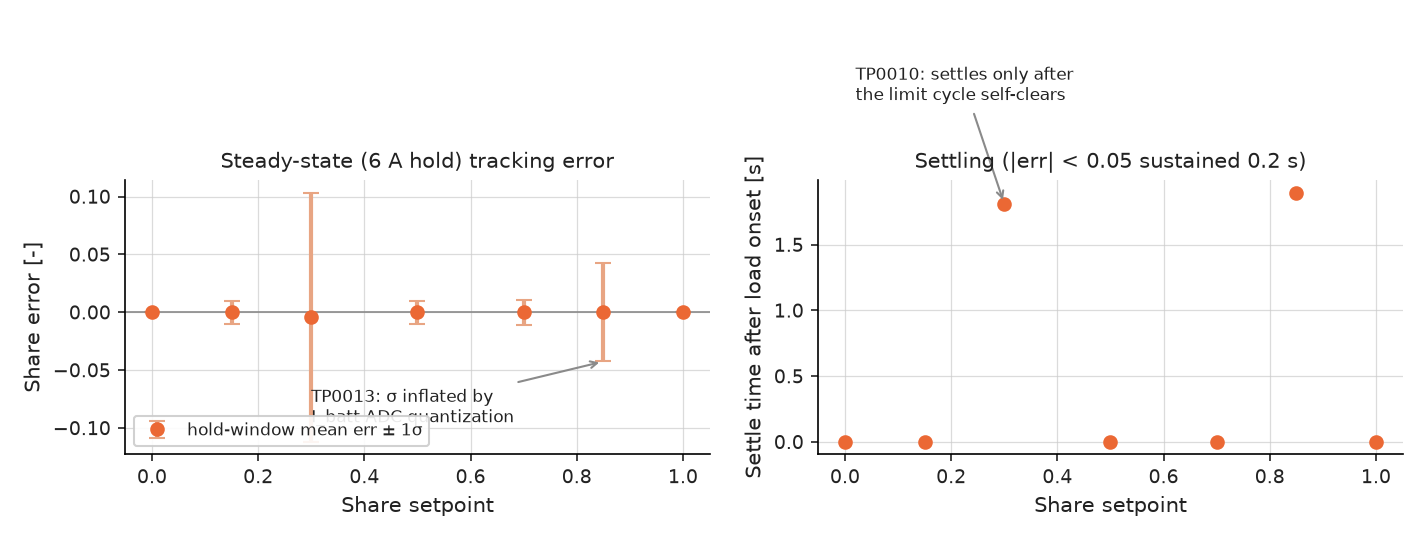
\includegraphics[width=\textwidth]{fig_sweep_summary.png}
\caption{Sweep summary. Left: hold-window tracking error is unbiased at every
setpoint; the two inflated $\sigma$ bars belong to the limit-cycle runs
(\code{TP0010}) and the quantization-corrupted high-share run (\code{TP0013}).
Right: settling time; interior and endpoint runs are within band at load onset,
while the two anomalous runs take $\approx$1.8--1.9\,s.}
\label{fig:summary}
\end{figure}

\begin{figure}[H]
\centering

\includegraphics[width=0.92\textwidth]{TP0007/currents_and_share.png}
\caption{Representative clean run (\code{TP0007}, $r^\ast=0.5$): symmetric channel
currents through the full trapezoid, share locked to the setpoint whenever total
current is above the measurement floor. The share excursions before load onset and
after load release are the known low-current region where the share ratio is
numerically undefined, not a control failure.}
\label{fig:tp0007}
\end{figure}

Actuator headroom, however, is \emph{asymmetric}. At $r^\ast=0.15$ the FC droop
command rides 0.85--0.91 (within $\approx$5\,\% of its ceiling) yet the run is the
fastest-settling of the sweep. The mirror case $r^\ast=0.85$ needs
$g_\mathrm{BT}\approx0.90$--$0.99$ \emph{and} $g_\mathrm{FC}$ pinned at its 0.175
floor for 85\,\% of the loaded window --- and misbehaves (Section~\ref{sec:tp0013}).
The usable share band is therefore not symmetric about 0.5: the FC-heavy side runs
out of authority first. This should inform the pending bench calibration of
$K_\mathrm{DROOP}$ and the droop-ratio band rather than being read as a controller
defect.

\section{The minority-channel dropout limit cycle}
\label{sec:limitcycle}

\subsection{Severe form: \code{TP0010}, $r^\ast=0.30$}

From $t=4.33$\,s to $6.15$\,s --- mid ramp-up, with the motor command between 4.3 and
6\,A but total channel current still below $\approx$1.2\,A --- the loop enters a
sustained relaxation oscillation with a median period of 58--59\,ms
($\approx$17\,Hz). Figure~\ref{fig:tp0010win} shows the full window;
Figure~\ref{fig:tp0010cyc} resolves individual cycles.

\begin{figure}[H]
\centering
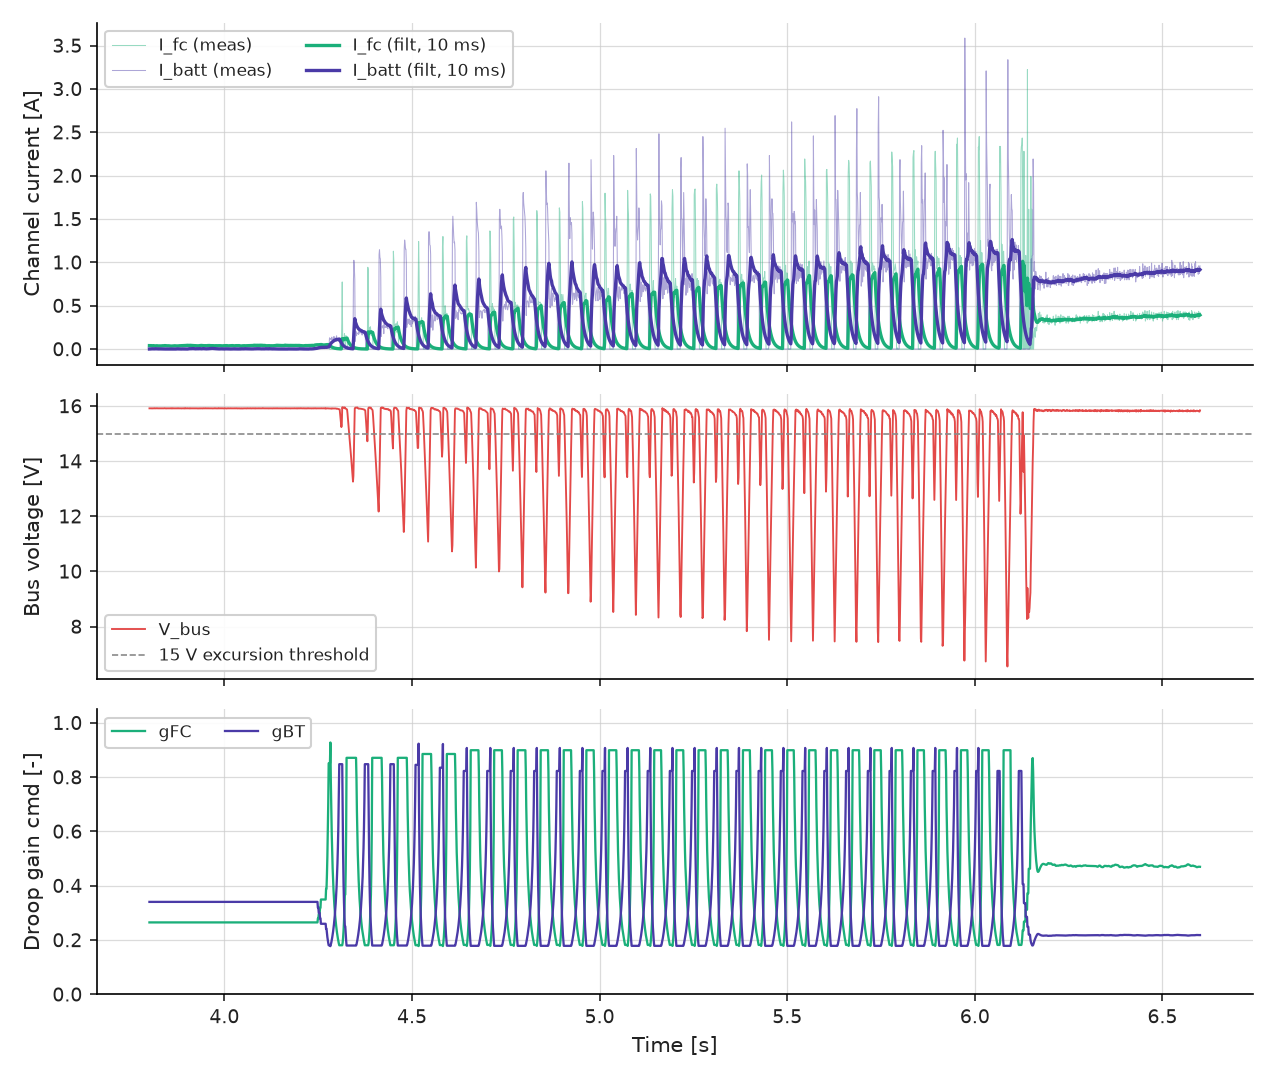
\includegraphics[width=0.95\textwidth]{fig_tp0010_window.png}
\caption{\code{TP0010} limit-cycle window. Top: channel currents alternate with
reconnect spikes growing to 3.6\,A as the load ramp deepens. Middle: 64 bus
excursions below 15\,V, reaching 6.55\,V; sag depth grows monotonically with the
commanded load. Bottom: the droop MDAC commands bang between their extremes in
antiphase. The cycle self-clears at $t=6.15$\,s once total current exceeds
$\approx$1.2\,A, and the remainder of the run is clean.}
\label{fig:tp0010win}
\end{figure}

\begin{figure}[H]
\centering
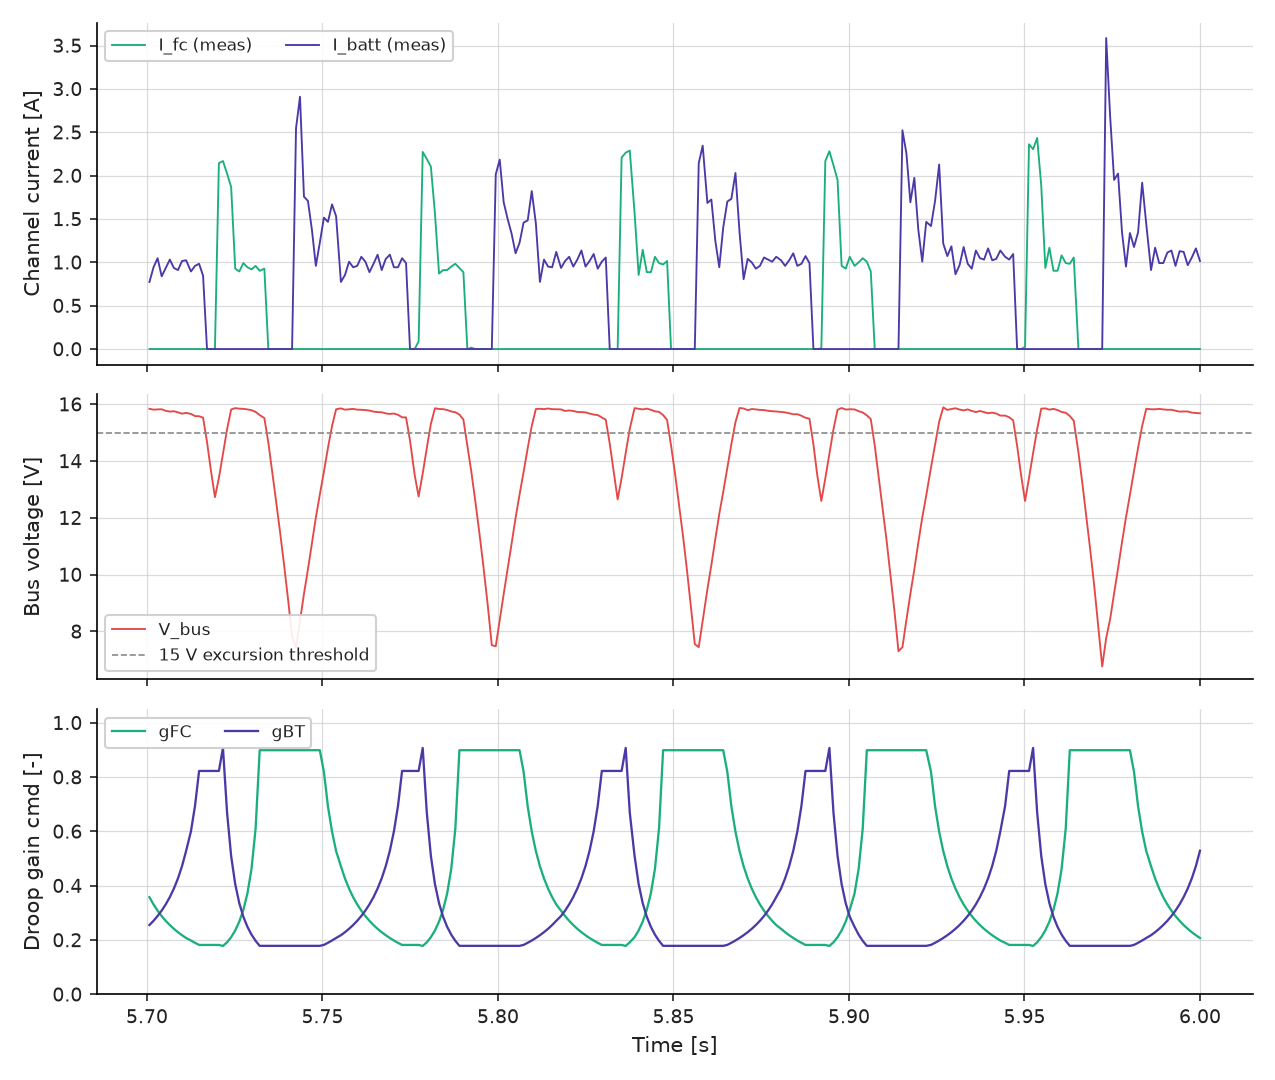
\includegraphics[width=0.95\textwidth]{fig_tp0010_cycle.png}
\caption{Five consecutive cycles of the \code{TP0010} limit cycle. The two channels
conduct \emph{mutually exclusively} (both conducting in only 0.1\,\% of samples);
each handoff includes a 10--18\,ms window in which \emph{both} channels read zero
current and the bus --- carrying only its $\approx$40\,$\mu$F of ceramics --- falls
as low as 6.5\,V before the incoming channel reconnects with a 2--3.6\,A spike.}
\label{fig:tp0010cyc}
\end{figure}

Three features deserve emphasis. First, the collapse is real and repeated: 64
excursions below 15\,V in 1.8\,s, with sag depth scaling with the commanded load
(13.3\,V at $I_\mathrm{cmd}=4.4$\,A down to 6.5\,V at 6\,A). Second, \emph{no fault
was raised}: the \code{BENCH\_TEST} build arms overvoltage checks only, and every
excursion is downward --- the event is invisible to \code{detectFaults()} as
currently configured on the bench. Third, the cycle is self-limiting in this run:
once the trapezoid pushes total current past $\approx$1.2\,A the loop converges and
the remainder of the run is indistinguishable from the clean runs
($\sigma=0.011$, no saturation). A brief re-entry occurs on the low-current tail at
$t\approx13.5$\,s.

\subsection{Mild form: \code{TP0013}, $r^\ast=0.85$}
\label{sec:tp0013}

The mirror-side asymmetric setpoint shows the same signature at 18.5--18.7\,Hz, but
as minority-channel (battery) dropout chatter without bus collapse
(Figure~\ref{fig:tp0013}): during both ramps the BT channel repeatedly falls to
exactly zero current (pinned there for 0.77\,s of the 1.5\,s ramp-up band and 1.36\,s
of the 2.1\,s ramp-down band), the measured share slams to 1, and $g_\mathrm{BT}$
rails before the channel snaps back. Bus disturbance is limited to
$\approx$100\,mV notches. The run never meets the strict settling criterion
($|e|<0.03$ for 200\,ms) anywhere; its mid-plateau is acceptable but has the worst
steady-state spread of the sweep.

\begin{figure}[H]
\centering
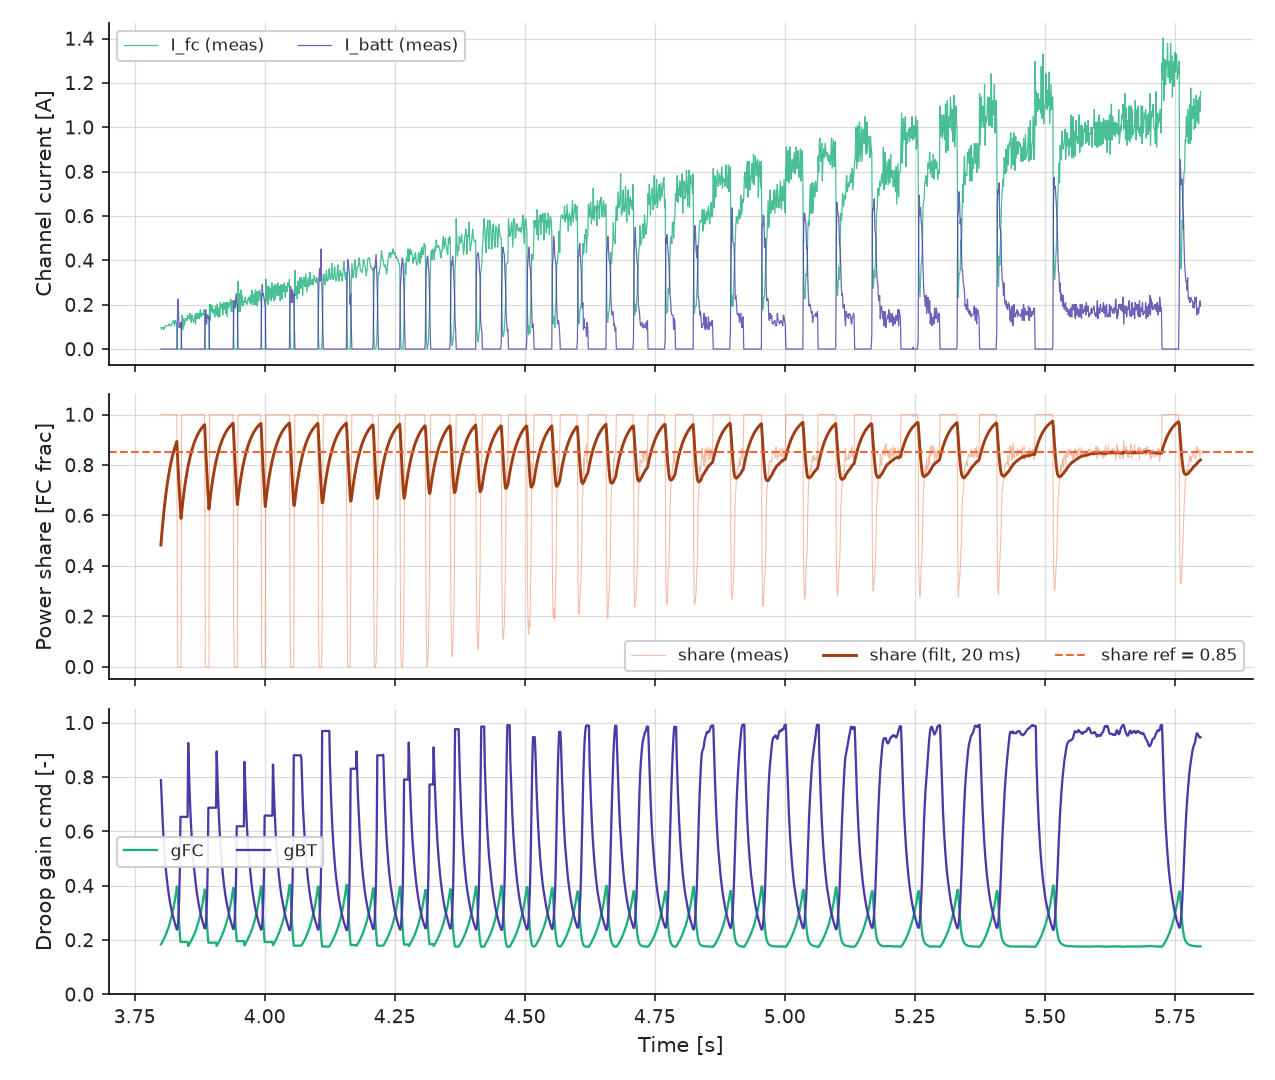
\includegraphics[width=0.95\textwidth]{fig_tp0013_dropout.png}
\caption{\code{TP0013} ramp-up dropout band. The BT channel (violet) repeatedly
drops out of conduction entirely; measured share (middle) saws between the setpoint
and 1.0 at $\approx$18.5\,Hz; $g_\mathrm{BT}$ (bottom) rails toward 1.0 on every
dropout while $g_\mathrm{FC}$ sits pinned at its 0.175 floor. Note the events thin
out as total current grows toward the plateau.}
\label{fig:tp0013}
\end{figure}

A separate measurement artifact compounds the picture at this setpoint: the
commanded battery current ($\approx$15\,\% of $\approx$0.5\,A $\approx$ 75\,mA) is
only $\approx$9 LSB of the 8.06\,mA current-sense quantization, and $I_\mathrm{BT}$
quantizes to exactly zero for 23\,\% of the loaded segment, pegging the computed
share at exactly 1.0. Excluding those samples reveals a genuine $-0.03$ share bias
at $r^\ast=0.85$ that the raw mean coincidentally cancels. Setpoint 0.85 at these
load levels is where the current-sense LSB begins to corrupt the share estimate
itself.

\subsection{Mechanism assessment}

The data support a \emph{starved-minority-channel dropout loop}: at low total
current, the droop command needed to hold the minority channel at a small fraction
pushes that channel out of conduction entirely (its RT1987 ideal diode blocks once
the droop-raised source characteristic falls below the bus); the measured share then
slams to 0 or 1, the controller drives both MDACs toward their rails, the starved
channel reconnects with a large spike, and the cycle repeats. This explains the
frequency similarity between the two runs, the mutual exclusivity, the confinement
to low total current, and the self-clearing once the minority channel's commanded
current rises above its conduction floor.

What that loop alone does \emph{not} explain is \code{TP0010}'s 10--18\,ms
\emph{both-channels-off} windows. Two candidates remain open, and the mechanism is
explicitly \textbf{unconfirmed} pending a scope capture:

\begin{enumerate}
\item both boosts are simultaneously droop-commanded out of conduction during the
crossover (a pure control-loop artifact of the antiphase rail-to-rail MDAC slew);
\item the RT1987 bus switches' short-circuit-protection cut/retry participates: the
58--59\,ms period is suspiciously close to the 64\,ms \code{tSCP\_RST} retry
fingerprint documented in the board's bring-up record (captures 9--10), and both bus
switches have carried 100\,nF soft-start capacitors since 2026-08-07, lengthening
every reconnect.
\end{enumerate}

A scope capture aimed at this question was taken on 2026-08-11 (capture~12 in the
bring-up record; Figure~\ref{fig:cap12}): a repeat of the \code{TP0010} condition
with VBUS, V-MOT, and the battery-channel INA monitored, single-shot trigger on VBUS
falling through 14\,V. It \emph{narrows} the question without closing it:

\begin{itemize}
\item \textbf{Confirmed: the events are total source-feed dropout windows.} VBUS and
V-MOT sag \emph{together} --- slow linear ramps of $\approx$3--4\,V over tens of
milliseconds at a 67.6\,ms cursor period (14.8\,Hz), each ended by a sharp recovery
synchronized with a $\approx$1\,A reconnect burst on the battery INA. Because the
motor switch conducts throughout, the bus rides the combined
$\approx$1--1.5\,mF motor+VESC capacitance during each window --- which is why the
decay is slow, and which independently corroborates the SD log's 10--18\,ms
both-channels-off reading.
\item \textbf{Ruled out: the VBUS$\rightarrow$V-MOT switch as a cutting element} (the
two nodes track through every dip).
\item \textbf{Still open: candidates (1) vs (2).} Both predict exactly this bus
signature, and the 67.6\,ms period is consistent with either (the RT1987 retry timer
is 64\,ms; the SD-log median was 58--59\,ms). The sharper discriminator, if needed:
probe a \emph{boost output} alongside VBUS during a dropout --- reconnect at the
voltage crossing indicates droop-commanded blocking, reconnect on a fixed 64\,ms
cadence indicates SCP.
\end{itemize}

Practically, the discrimination no longer gates the fix: both surviving candidates
are downstream of the droop loop railing both MDACs antiphase, so the mitigation set
of Section~\ref{sec:conclusions} (feasibility-gated integrator hold, MDAC slew
limiting) is the correct next step under either mechanism.

\begin{figure}[H]
\centering
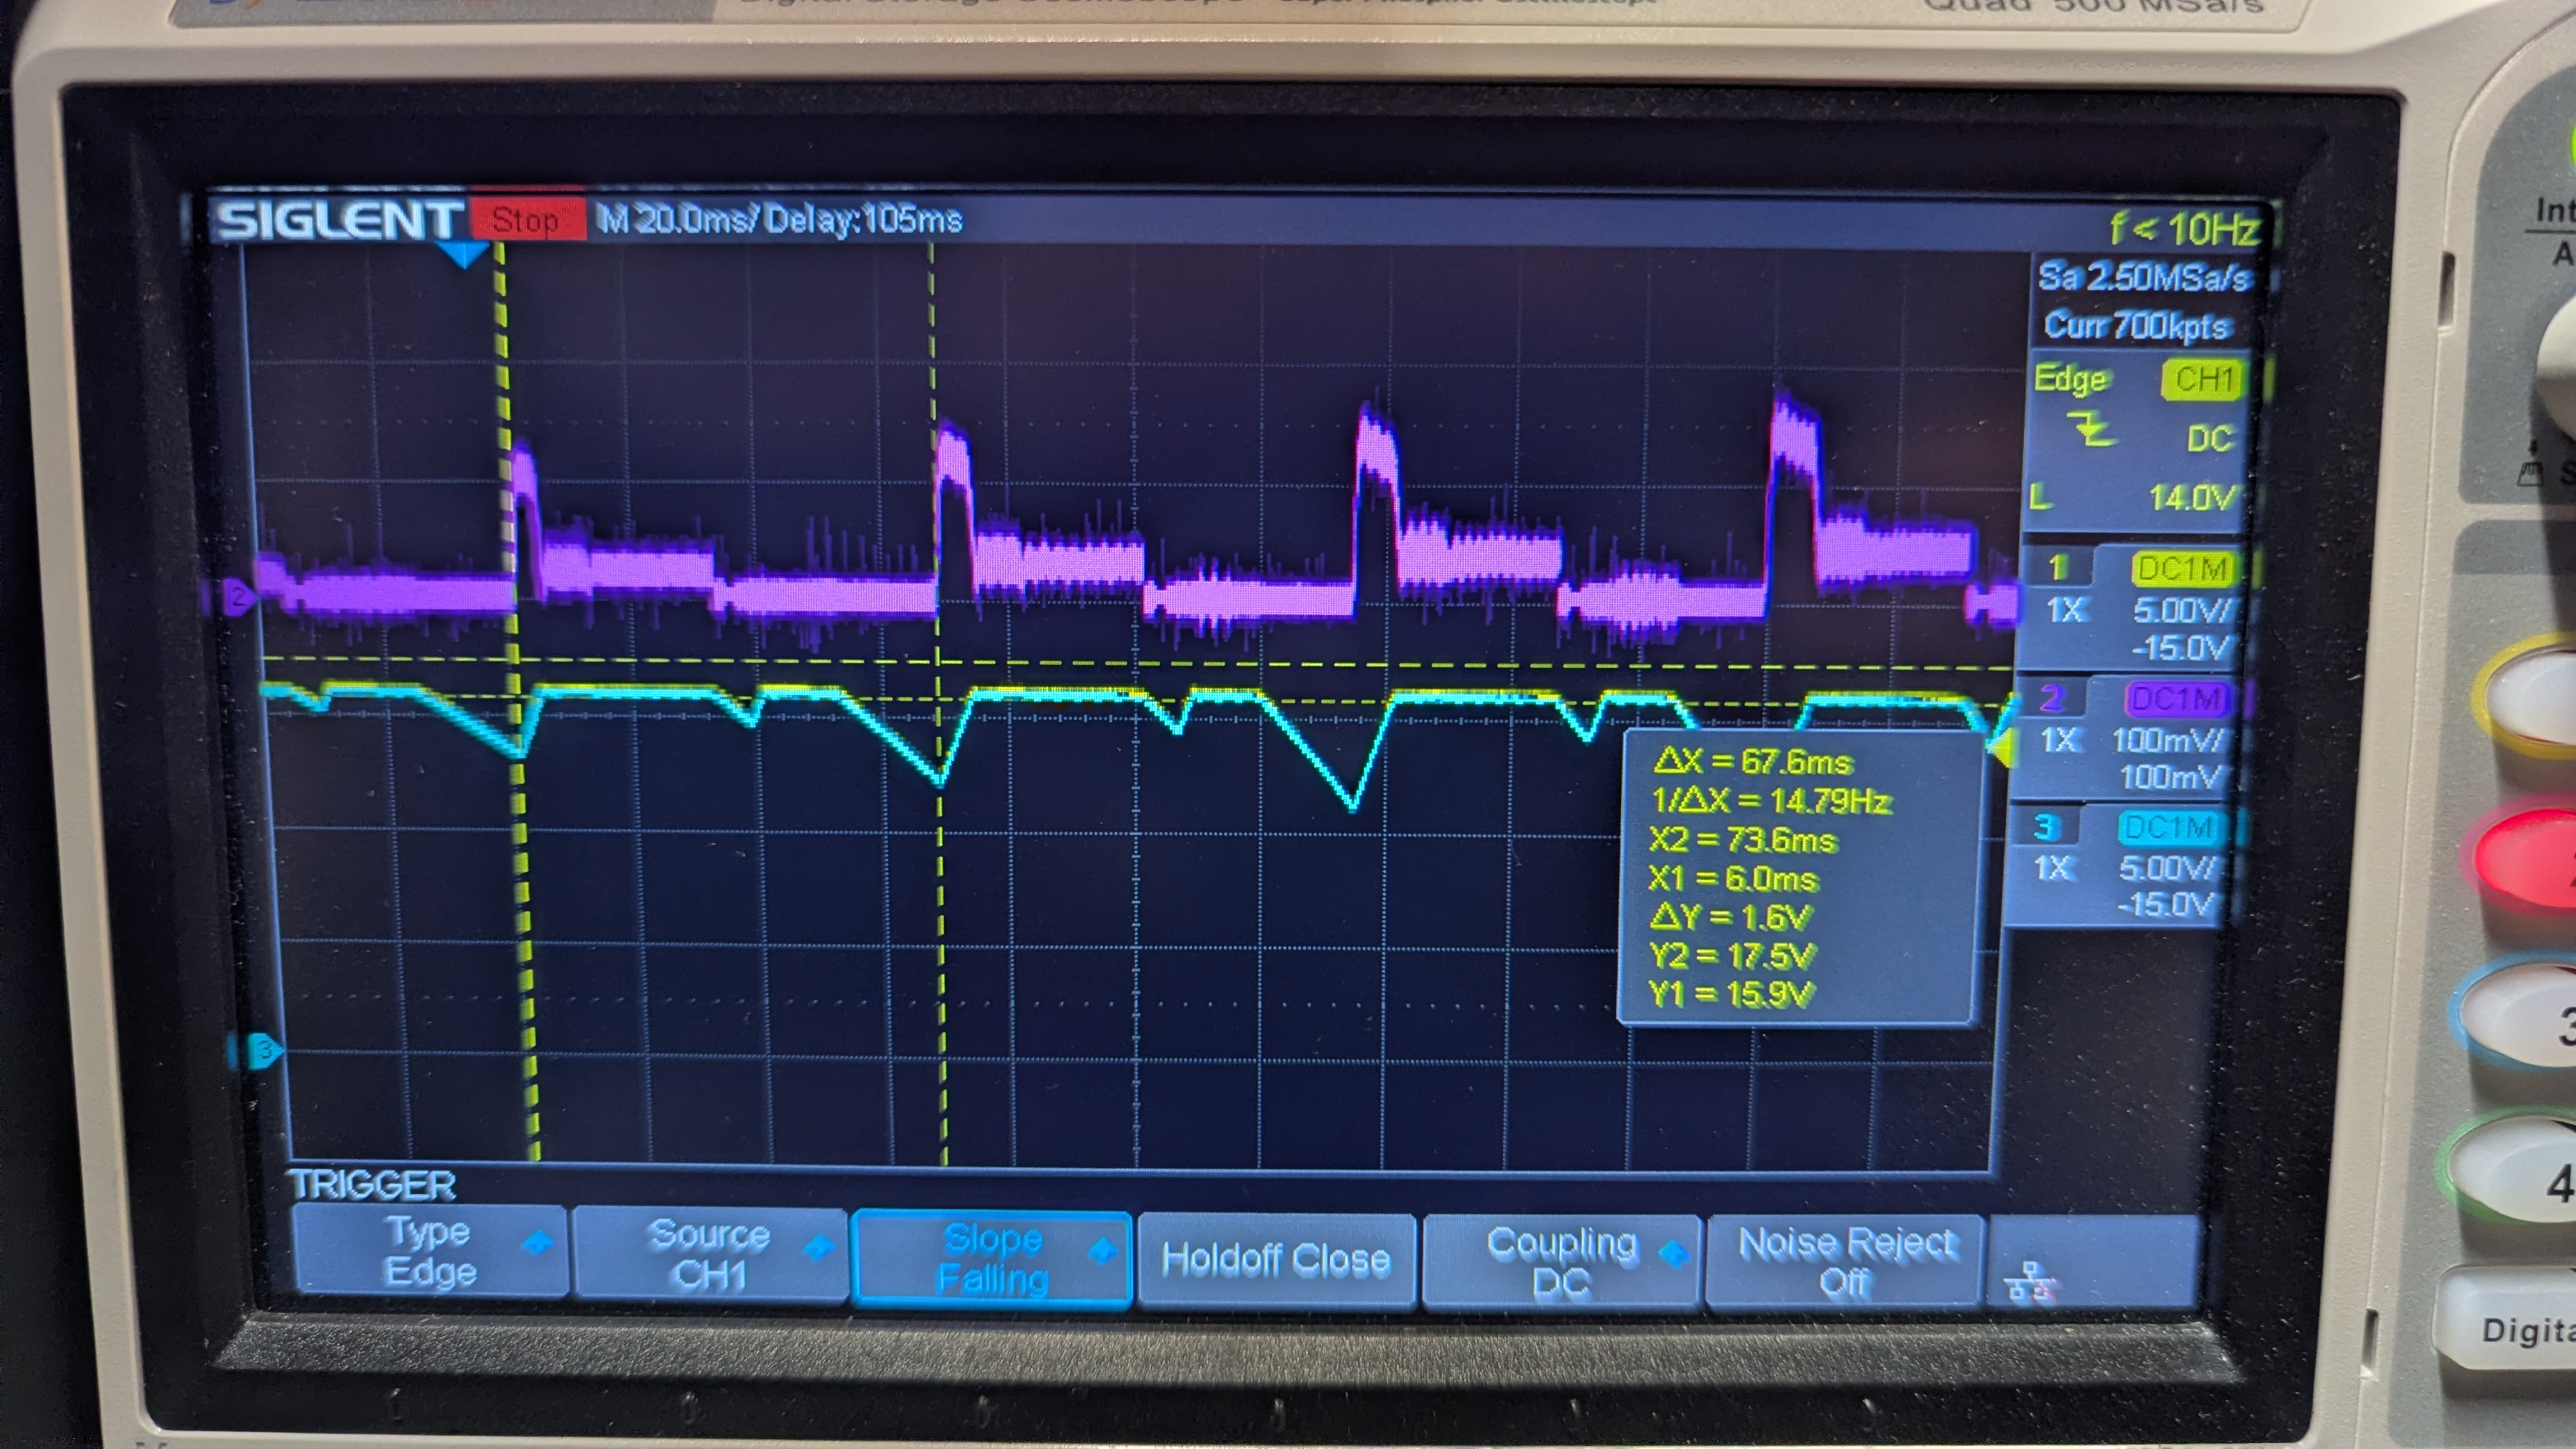
\includegraphics[width=0.9\textwidth]{capture12.jpg}
\caption{Capture 12 (2026-08-11): \code{TP0010}-condition repeat, 20\,ms/div.
CH1 VBUS (yellow, 5\,V/div) and CH3 V-MOT (blue, 5\,V/div) overlap and sag together
in $\approx$3--4\,V sawtooth ramps at a 67.6\,ms period (cursors); CH2 battery INA
(purple, 1\,A/div) shows the dropout--reconnect-spike--conduction pattern
synchronized with the voltage recoveries. The flat yellow line near 15.9\,V is the
Y1 measurement cursor, not the VBUS trace.}
\label{fig:cap12}
\end{figure}

\subsection{Why a nondestructive event matters}

Each reconnect is a load-dump-class transient sourced by a boost converter, on a
board whose failure history (five destroyed TPS61288 converters) traces to exactly
this event class. The per-event energy here is far below the destructive episodes,
and both boost converters carry the validated hot-loop bodge capacitors, which
bounds the known overshoot mechanism --- but \code{TP0010} delivered $\approx$33
collapse/reconnect events in under two seconds, a duty cycle the power stage has
not been characterized under. Capture~12 confirms the whole bus --- sources to VESC
--- rides each dropout's decay, so until the firmware mitigation lands, repeated
runs at $r^\ast\approx0.3$ with ramping load should be treated as a known stressor. The
event is logged in \code{docs/boost-bringup-debug.md} with a corresponding safety
rule and follow-up item.

\section{Secondary observations}

\paragraph{Low-load integrator windup (expected, mild).} This firmware predates the
planned minimum-load integrator hold. During the 30--41\,\% of each run spent below
the share-measurement floor, the gain commands drift toward their extremes
(0.90--0.99), producing load-return transients of up to $-0.85$ / $+0.70$ share
error with 0.5--1.9\,s recovery --- worst in exactly the two runs that also limit-cycled.
Note, however, that the limit cycle itself lives at total currents up to
$\approx$1.2\,A, an order of magnitude above the planned 75\,mA hold threshold: the
pending fix as parameterized would \emph{not} have suppressed it.

\paragraph{Controller state carries across runs.} Each run's initial MDAC pair
equals the previous run's final value (only \code{TP0007}, first after boot, starts
from zero). This contaminates each run's entry transient and should be reset at
profile entry.

\paragraph{Run-order drift.} At the identical 6\,A motor command, mean bus current
during the hold climbs monotonically with session order --- 1.20\,A
(\code{TP0007}) to 1.72\,A (\code{TP0013}), $+44$\,\%
(Figure~\ref{fig:runorder}) --- consistent with battery depletion and/or motor
heating across the session. Cross-run comparisons are therefore made at a slowly
drifting operating point; future sweeps should interleave or randomize setpoint
order.

\begin{figure}[H]
\centering
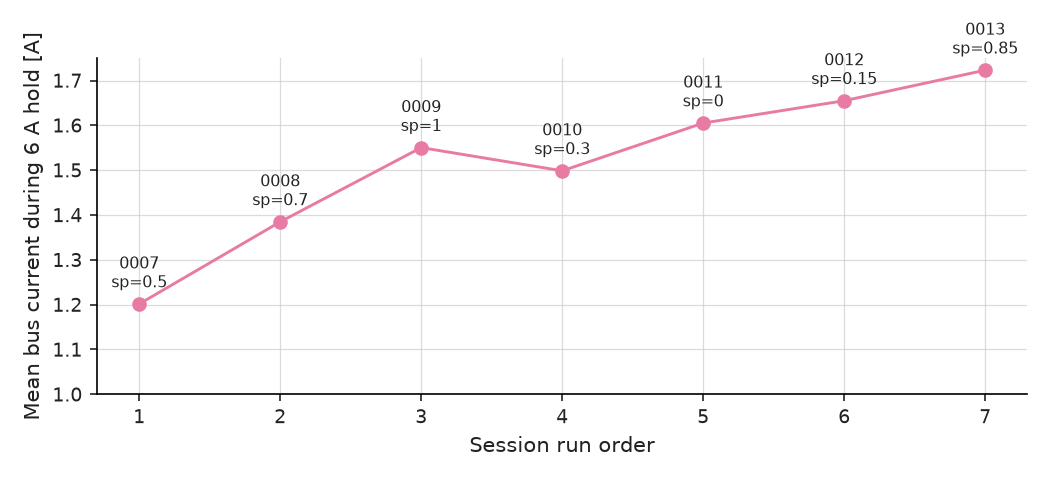
\includegraphics[width=0.8\textwidth]{fig_run_order.png}
\caption{Session drift: mean bus current during the 6\,A hold vs.\ run order. The
+44\,\% monotonic climb tracks session order, not setpoint.}
\label{fig:runorder}
\end{figure}

\paragraph{Comparison to the earlier runs.} The five earlier captures
(\code{PS0001}--\code{PS0003} share-step profiles, \code{TP0004}--\code{TP0005}
trapezoids at $r^\ast=0.5$) show clean step tracking (0.2/0.5/0.8 plateaus, settling
within $\approx$1\,s, no overshoot) and clean trapezoid tracking at 0.5,
respectively. The new sweep reproduces that behavior at every operating point the
old runs covered --- there is no regression. The limit cycle appears only at
asymmetric setpoints the earlier campaign never visited. (The earlier runs used
less analog averaging; noise-level comparisons between the two groups are
deliberately out of scope.)

\section{Fix-validation sweep (firmware v3)}
\label{sec:validation}

\subsection{Mitigation set and sweep design}

Following the analysis above, firmware~v2/v3 added three mitigations to the share
loop. First, a \emph{setpoint governor} clips the effective in-band setpoint so the
commanded minority-channel current stays at or above
$I_\mathrm{min}=\code{SHARE\_MINORITY\_I\_MIN\_A}=0.20$\,A, computed against a
low-pass estimate of total current; below $2I_\mathrm{min}$ of filtered total the
effective setpoint collapses to 0.5. Setpoints outside the droop band $[0.15,0.85]$
bypass the governor, on the design assumption that the channel-cutoff path owns
them. Second, a \emph{droop-ratio slew limit} of 0.02 per control tick replaces the
rail-to-rail MDAC slams of Figure~\ref{fig:tp0010win}. Third, share-controller
state is \emph{reset at every profile start}, removing the cross-run contamination
of Section~5.

The validation campaign ran on firmware~v3 using the automated \code{T}-sweep
extension: 25 trapezoid runs (\code{TP0014}--\code{TP0038}), identical
\code{T 6 3 1} profile, one run per setpoint on the ladder $\{0, 0.12, 0.15, 0.18,
0.20, 0.225, 0.25, 0.30, \ldots, 0.84, 0.85, 0.87, 1.0\}$, with dense placement at
both band edges to map the failure boundary. Two \code{W} combined profiles
(\code{WP0039}, \code{WP0040}) exercised the loop under a \emph{moving} setpoint
and load. All trapezoid captures are complete with clean trailers;
\code{WP0039} is truncated (Section~\ref{sec:wp0039}).

\subsection{Result: the limit cycle is eliminated across the governed band}

Figure~\ref{fig:valsummary} summarizes the ladder. Every setpoint from 0.18 to
0.85 --- including 0.30 and 0.85, the two original failure points --- runs with zero
dropout events, a flat bus (run minimum 15.72\,V against a 15.9\,V rail), and
hold-window bias below $10^{-4}$ with $\sigma=0.009$--$0.017$. At the original
severe point 0.30 (\code{TP0021}), the comparison against \code{TP0010} is: 64
collapse events to zero; bus minimum 6.55\,V to 15.73\,V; peak reconnect current
3.6\,A to 0.74\,A.

\begin{figure}[H]
\centering
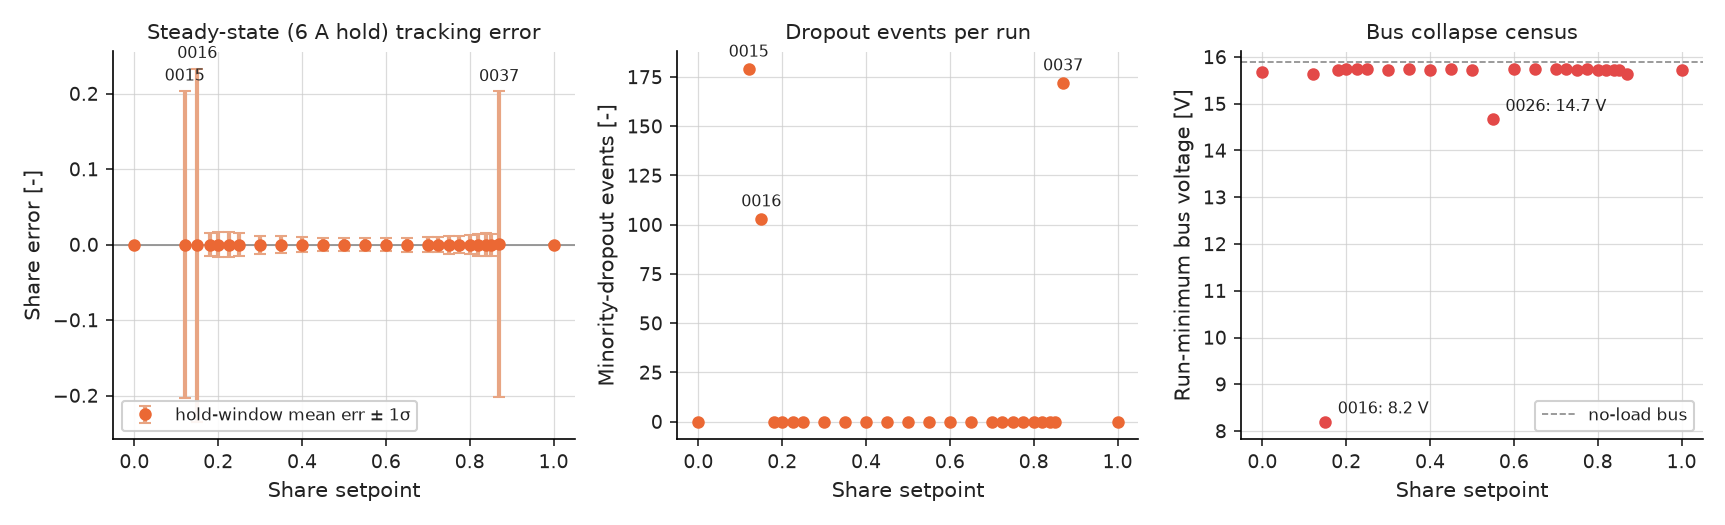
\includegraphics[width=\textwidth]{fig_valsweep_summary.png}
\caption{Validation-sweep summary, \code{TP0014}--\code{TP0038} (firmware v3).
Left: hold-window tracking error remains unbiased at every setpoint; the three
inflated $\sigma$ bars are the residual failure runs. Center: hysteretic
dropout-event count --- only 0.12, 0.15, and 0.87 cycle; the deep out-of-band
endpoints 0 and 1 are clean latched cutoffs. Right: run-minimum bus voltage;
only \code{TP0016} (0.15) collapses the bus.}
\label{fig:valsummary}
\end{figure}

The governor's mechanism is directly observable in the logs. In every clean
asymmetric run the minority-channel current is pinned at 0.204--0.214\,A --- the
0.20\,A floor held to within 5\,\% --- across a threefold span of total current,
then released at the predicted crossover $I_\mathrm{tot}=I_\mathrm{min}/r^\ast$
plus the load-filter lag. The collapse-to-0.5 plateau below 0.40\,A filtered total
appears as a distinct shelf in every ramp. The slew limiter is respected exactly in
all 27 runs (maximum per-record ratio step 0.0200) and saturates for substantial
stretches, confirming it is load-bearing.

The moving-setpoint run \code{WP0040} (Figure~\ref{fig:wp0040}) extends the
validation to simultaneous setpoint and load steps: across all sixteen table
regions, the measured share tracks the \emph{reconstructed governed setpoint} with
residuals at or below $2\times10^{-3}$, including three regions where the governor
clips a 0.65 command down to 0.54--0.57 at low current and two regions where it
collapses a 0.30/0.65 command to 0.5. The apparent tracking ``errors'' against the
raw table setpoint are therefore entirely commanded governor action. Region
boundaries traverse ratio steps of up to 0.34 in about 20 slew-limited ticks with
$\approx$0.06 overshoot and no bus disturbance beyond 0.20\,V.

\begin{figure}[H]
\centering
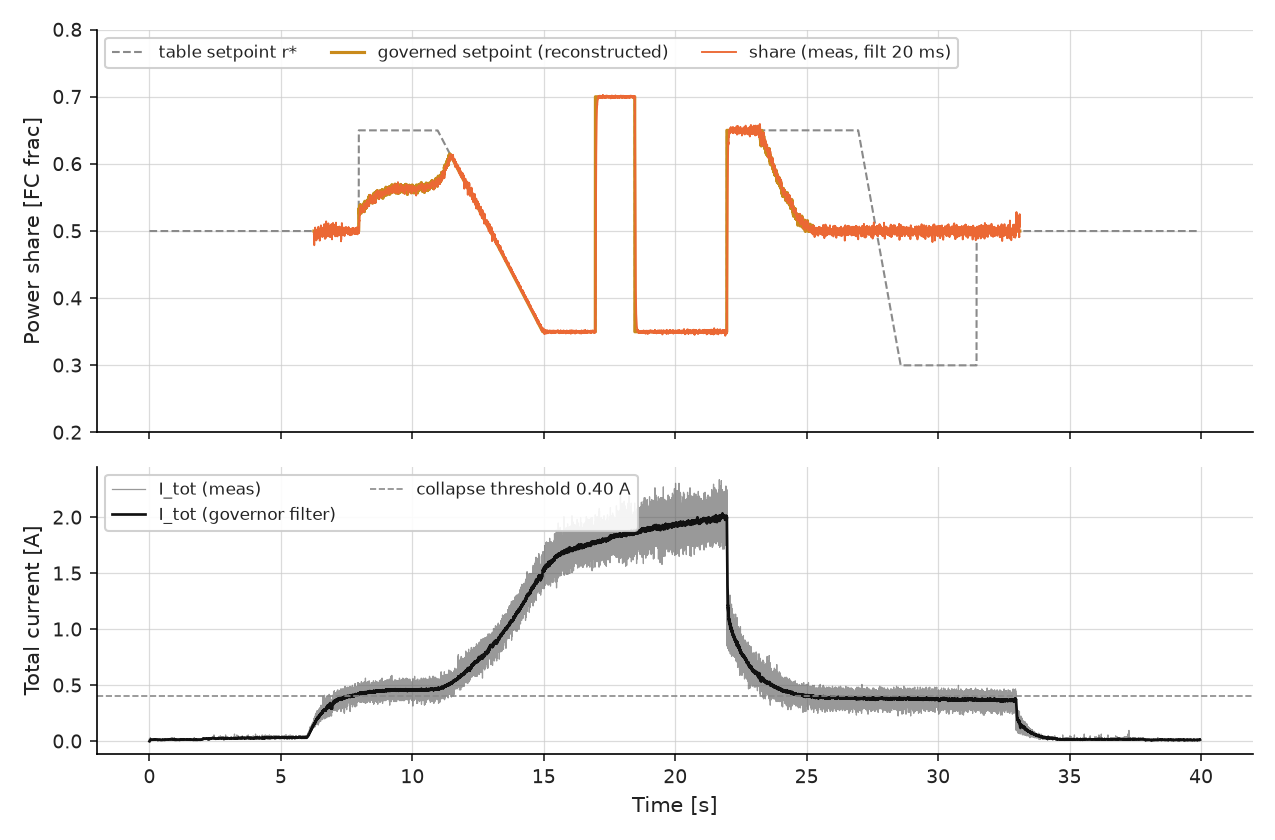
\includegraphics[width=0.95\textwidth]{fig_wp0040_governor.png}
\caption{\code{WP0040} (moving setpoint and load): measured share (orange) against
the raw table setpoint (dashed) and the governed setpoint reconstructed from the
firmware's clip law (mustard). The measured share follows the governed command
everywhere the share is measurable; the flat 0.5 stretches at $t=25$--33\,s are the
designed collapse below $2I_\mathrm{min}$ of filtered total current, not tracking
failure.}
\label{fig:wp0040}
\end{figure}

\subsection{Residual failure at the in-band boundary: \code{TP0016}, $r^\ast=0.15$}
\label{sec:tp0016}

The single in-band failure is the band-edge setpoint itself.
\code{TP0016} ignites the limit cycle at $t=6.14$\,s --- the precise instant the
governor releases, when total current grows past
$I_\mathrm{min}/0.15=1.33$\,A and the commanded minority current passes down
through 0.20\,A. Zero dropout events occur before that instant; the cycle then runs
continuously through the hold (56 events at 19\,Hz, bus intact) and deepens through
the ramp-down (Figure~\ref{fig:tp0016}): 44 bus excursions below 15\,V, reaching
\textbf{8.20\,V}, with 2.4\,A reconnect spikes and simultaneous
both-channels-at-zero windows --- the same total source-feed dropout signature as
\code{TP0010}, at roughly three-quarters its event count and 1.6\,V shallower
minimum.

\begin{figure}[H]
\centering
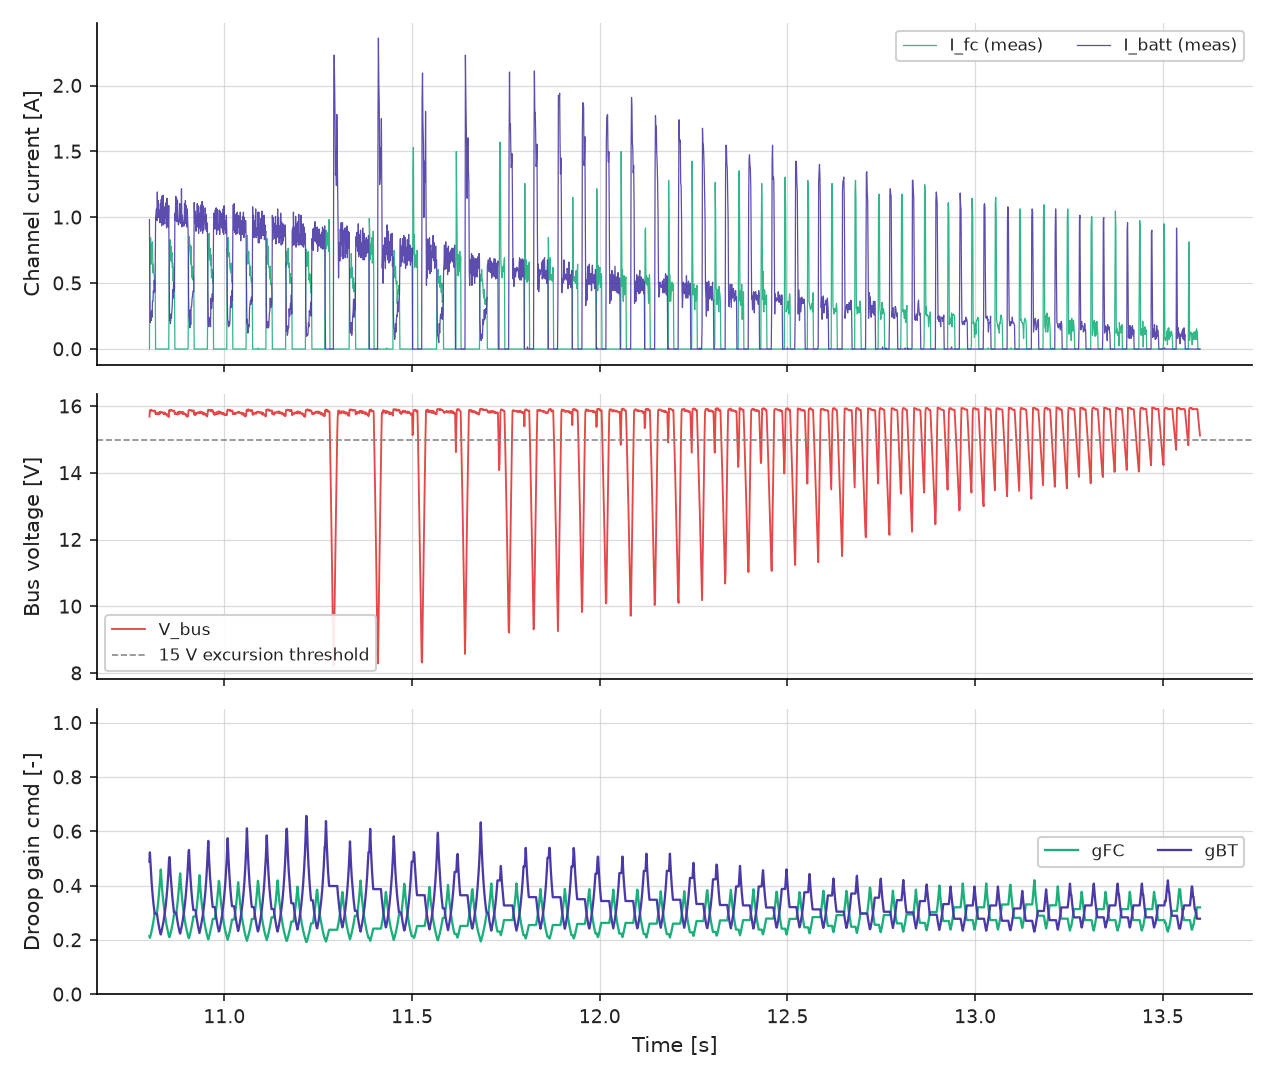
\includegraphics[width=0.95\textwidth]{fig_tp0016_window.png}
\caption{\code{TP0016} ($r^\ast=0.15$) ramp-down window. The limit cycle survives
at the in-band boundary: mutually exclusive conduction with reconnect spikes to
2.4\,A (top), bus collapse deepening to 8.2\,V as commanded current falls (middle),
and the droop-gain commands cycling in antiphase --- now confined to 0.2--0.65 by the
slew limiter rather than slamming rail-to-rail as in fw~0 (bottom).}
\label{fig:tp0016}
\end{figure}

Two independent quantities corner this setpoint. First, the governor floor at the
hold's 1.63\,A is $0.20/1.63=0.122$, below the setpoint --- so the governor
correctly declines to clip, and the commanded minority current (0.245\,A) is
evidently still inside the dropout region: the empirical conduction floor lies
between 0.245\,A (cycles, this run) and 0.29\,A (\code{TP0017} at $r^\ast=0.18$,
clean). $I_\mathrm{min}=0.20$\,A therefore sits \emph{on} the failure boundary
rather than above it. Second, the commanded droop ratio in the hold tracks the
setpoint to within 0.003 in every clean run, so $r^\ast=0.15$ parks the actuator
directly on the \code{DROOP\_R\_MIN} rail --- \code{TP0016}'s minimum hold margin to
the rail is $+0.0005$, inside the 0.01 cutoff re-entry hysteresis. Ignition
coincides with the ratio touching the rail. Raising $I_\mathrm{min}$ alone
addresses the first constraint; the second argues for narrowing the usable in-band
span to approximately $[0.18, 0.82]$ independent of load.

\subsection{The ungoverned setpoint window: \code{TP0037}, $r^\ast=0.87$}
\label{sec:gap}

\code{TP0037} exposes a structural gap between the two mitigation paths. The
setpoint 0.87 is outside the droop band, so the governor is bypassed by design ---
the cutoff path is assumed to own it. But the cutoff fires on the \emph{controller
output} $r$, not on the setpoint, and the plant needs only $r\approx0.84$ to
realize a share of 0.87: extrapolating the clean runs' hold-window ratios
(0.770/0.790/0.810/0.821 at $r^\ast=0.80$/0.82/0.84/0.85) puts the required ratio
just \emph{below} the 0.85 cutoff threshold. The measured ratio confirms it:
maximum 0.789, never crossing (Figure~\ref{fig:tp0037}, bottom). Setpoint 0.87 is
therefore governed by nothing and cut off by nothing, and it runs the original
limit cycle unmitigated: 172 dropout--reconnect cycles at 19.5\,Hz, the BT channel
off the bus for $\approx$70\,\% of all loaded time at every current level ---
unlike fw~0, it does \emph{not} self-clear above 1.2\,A, because the ungoverned
commanded minority current (0.13 of total) stays below the conduction floor at
every point of this profile. Electrical severity stays low (bus ripple 0.33\,V,
spikes to 1.1\,A), but the cycle is continuous. The unprotected window is
approximately $0.85<r^\ast\lesssim0.88$, with a mirror on the low side --- where it
is compounded by a second mechanism: at $r^\ast=0.12$ (\code{TP0015}) the
controller output \emph{does} cross the low threshold, the cutoff opens the FC
switch, but the standing share error then winds the ratio back over the re-entry
hysteresis and the loop \emph{hunts} --- duty-cycling \code{FC\_BUS\_ENABLE} at
19.8\,Hz, about 190 ideal-diode switch cycles per 13\,s run. The deep endpoints 0
and 1 (\code{TP0014}, \code{TP0038}) latch cleanly, because there the realized
share equals the setpoint and the error vanishes: the hysteresis never re-arms.

\begin{figure}[H]
\centering
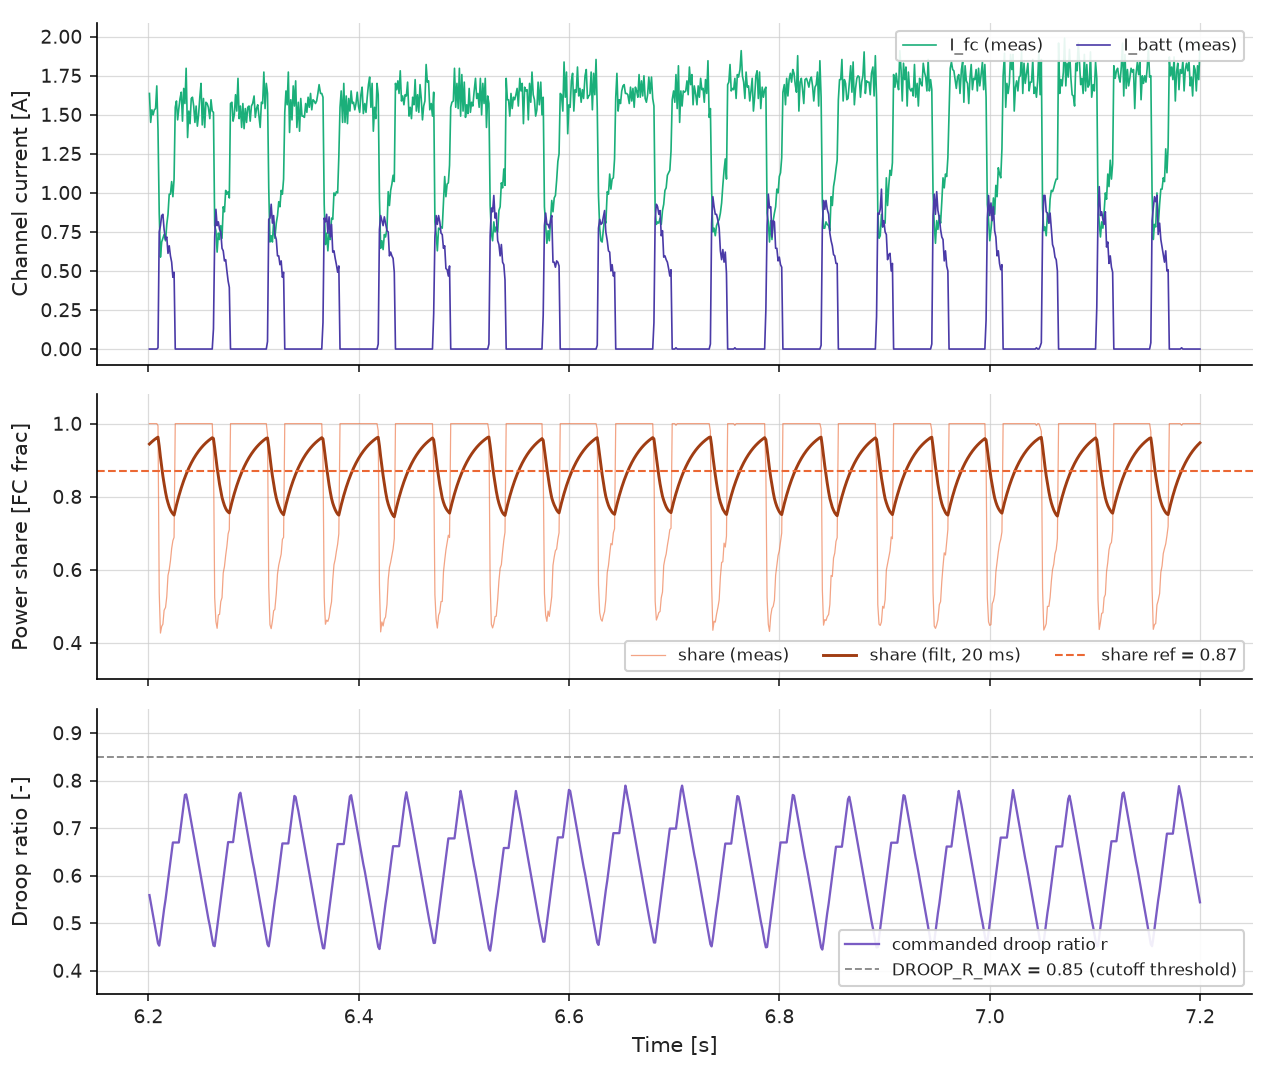
\includegraphics[width=0.95\textwidth]{fig_tp0037_gap.png}
\caption{\code{TP0037} ($r^\ast=0.87$) during the 6\,A hold: the unmitigated limit
cycle in the ungoverned window. The BT channel duty-cycles at 19.5\,Hz (top), the
filtered share saws around the setpoint (middle), and the commanded droop ratio
sawtooths between 0.45 and 0.79 --- never reaching the 0.85 cutoff threshold
(dashed, bottom), so neither mitigation path ever engages.}
\label{fig:tp0037}
\end{figure}

\subsection{\code{WP0039}: a brownout-terminated total-dropout ratchet}
\label{sec:wp0039}

\code{WP0039} (the first \code{W} combined profile, $I_\mathrm{max}=5$\,A) is the
campaign's one destructive-class event. The run is quiescent for 11.8\,s --- total
channel current 0.03--0.08\,A despite motor commands up to 3.4\,A, indicating the
motor was not accepting load (cause unconfirmed; a VESC in its brownout band would
fit) --- and then enters a 34\,Hz total source-feed dropout cut/retry cycle: both
channels drop to zero simultaneously, the motor-node capacitance
($\approx$1.6\,mF inferred from the decay slope) discharges at $\approx$465\,V/s,
and one channel reconnects with a 1.4--3.2\,A spike (Figure~\ref{fig:wp0039}). The
sag floor deepens monotonically from 13.9\,V to 7.6\,V over 89 cycles in 2.7\,s,
after which the bus enters free-fall and the log truncates mid-sample with no
trailer --- the signature of the board-powered Teensy browning out, not of an
operator stop. No fault was latched at any point: the \code{BENCH\_TEST} build arms
overvoltage only, so 0.87\,s of sub-14\,V bus and $\approx$90 load-dump reconnects
were invisible to \code{detectFaults()}. This is the capture-10/-12 event class
(total source-feed dropout ratchet) rather than the minority-channel cycle the
governor targets. One trigger correlation deserves a scope-armed re-entry: the
share loop sat frozen below its 75\,mA minimum-load threshold for the whole
quiescent stretch, unfroze at $t=11.75$\,s with a large standing error, and
traversed the droop ratio at the full slew rate ($0.734\rightarrow0.394$ in
$\approx$40\,ms) --- the first total dropout followed within 40\,ms.

\begin{figure}[H]
\centering
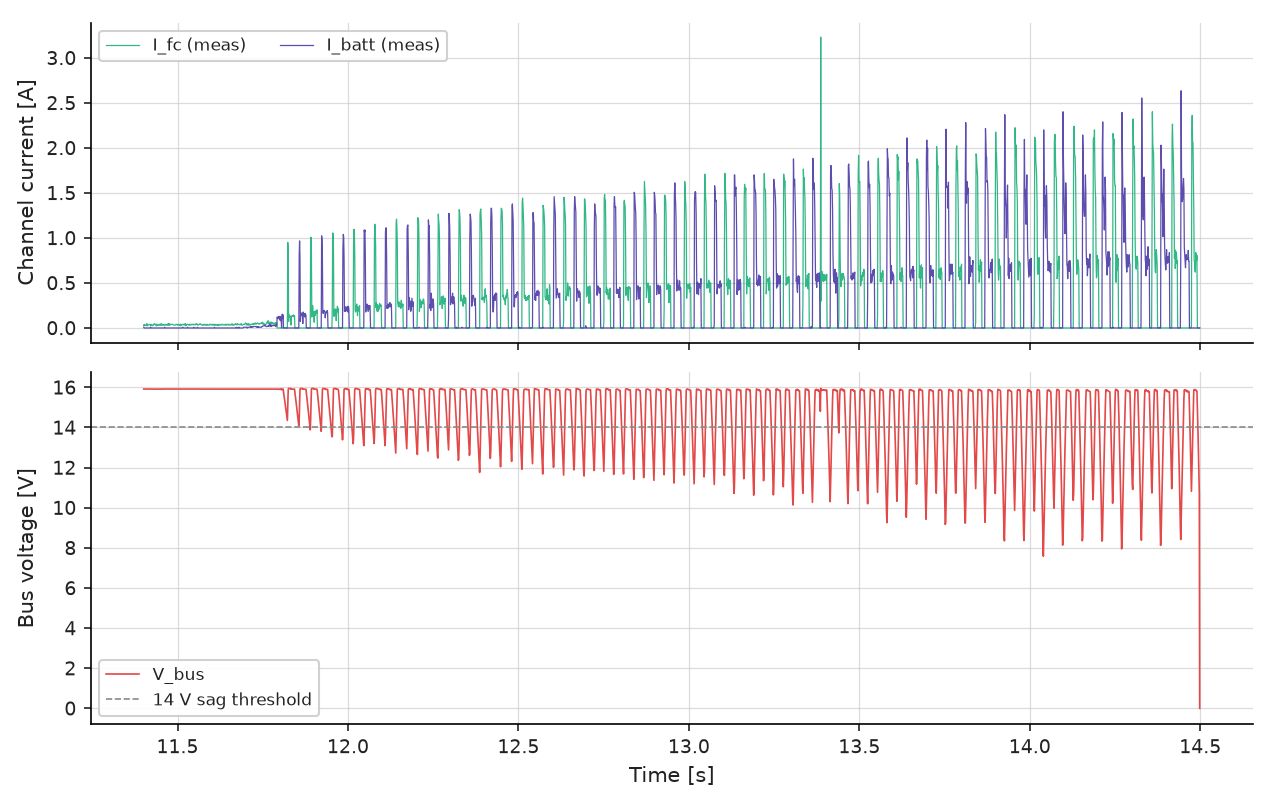
\includegraphics[width=0.95\textwidth]{fig_wp0039_ratchet.png}
\caption{\code{WP0039} final 3\,s. Top: both channels drop out together and
alternate 1.4--3.2\,A reconnect spikes at 34\,Hz. Bottom: the sag floor ratchets
monotonically from 13.9\,V to 7.6\,V, then the bus free-falls and the log truncates
mid-decay (no trailer) --- consistent with an MCU brownout. \code{fault\_flags}
remained zero throughout.}
\label{fig:wp0039}
\end{figure}

\subsection{Secondary observations from the validation campaign}

\paragraph{\code{TP0026} transient.} The $r^\ast=0.55$ run shows one brief
total-dropout burst in the ramp-down tail: three cycles at $\approx$26\,Hz over
71\,ms at $I_\mathrm{cmd}\approx1.2$\,A, with a single bus notch to 14.67\,V. It is
the same event class at roughly two orders of magnitude lower dose and did not
recur at any neighboring setpoint; it is flagged for the boundary-mapping session
rather than treated as a validation failure.

\paragraph{First-write MDAC step.} \code{WP0040} booted with both MDACs at code
zero until the share loop's first unfreeze at $t=6.05$\,s, whose first write is a
$\approx$0.5 ratio jump that bypasses the slew limiter (it originates from the
one-shot actuation path). Profile-entry reset does not force an MDAC write; runs
inheriting gains from a prior run do not show the step.

\paragraph{Effective sample rate.} Both campaigns log at $\approx$862--875\,Hz
(median interval 1.15--1.16\,ms) against a 1\,kHz nominal, with the decoder
reporting zero missed periods --- so the control tick itself, not the logger, runs
$\approx$14\,\% slow. If confirmed, the effective slew limit is $\approx$17\,$\mathrm{s^{-1}}$
rather than the documented 20\,$\mathrm{s^{-1}}$; the discrepancy is flagged for a
firmware timing check.

\section{Second validation sweep (firmware v4)}
\label{sec:v4}

\subsection{Mitigation set and sweep design}

Firmware~v4 implements the three actions recommended in
Section~\ref{sec:conclusions} items~4--6. First, the governor floor
\code{SHARE\_MINORITY\_I\_MIN\_A} rises from 0.20 to 0.30\,A, above the
$(0.245, 0.29)$\,A conduction bracket of Section~\ref{sec:tp0016}; the
collapse-to-0.5 threshold rises to 0.60\,A of filtered total current
accordingly. Second, the governor/cutoff structural gap closes with a
\emph{setpoint-latched cutoff}: any setpoint outside $[0.15, 0.85]$ immediately
opens the starved channel's bus switch, freezes the share loop, and releases only
on setpoint re-entry --- replacing the output-ratio hysteresis that hunted at
$r^\ast=0.12$ and never fired at 0.87. Third, a persistence-filtered
bus-undervoltage fault (\code{FAULT\_UV\_BUS}: 12.0\,V limit, 10\,ms plus three
consecutive samples, 5\,ms gap guard) is armed under \code{BENCH\_TEST}.

The campaign comprises a 28-point trapezoid ladder (\code{TP0041}--\code{TP0068},
identical \code{T 6 3 1} profile) spanning $r^\ast$ from 0 to 1.0 with dense
placement at both band edges and across 0.67--0.85, and five \code{W} combined
profiles
(\code{WP0069}--\code{WP0073}, $I_\mathrm{max}=6$\,A) that ladder the share-clip
bound $b$ from 0.35 down to 0.20. Six trapezoid runs latched
\code{ERR\_UV\_BUS} and two \code{W} runs truncated without a trailer; the
session structure matters for their interpretation. The first fault
(\code{TP0053}, $r^\ast=0.70$) struck on the thirteenth consecutive run of one
automated session; the four bisection runs that followed (0.67--0.73) each ran on
a fresh boot within 30\,s of the previous fault's power cycle. A source-state
confound is therefore not excluded by the run order alone, but the bus at a fixed
2\,A ramp point is 15.919--15.926\,V across all 33 runs, and the mechanism
evidence below does not require one.

\subsection{The firmware v3 failure points are closed}

Figure~\ref{fig:v4summary} summarizes the ladder. All three residual failure
classes of Section~\ref{sec:validation} are eliminated:

\begin{itemize}
\item \textbf{Out-of-band hunting.} All seven out-of-band setpoints
(0--0.12 and 0.88--1.0) latch once at the first loop tick and never cycle: the
droop gains are constant from the first to the last sample, the cut channel's
current is pinned at the ADC noise floor, and the hysteretic event count is zero.
At $r^\ast=0.12$ the comparison against firmware~v3 is 179 switch cycles to
zero; at 0.88--0.90 (the former ungoverned window) it is a continuous 19.5\,Hz
limit cycle to a static latch. \code{TP0066} (0.88) shows the one artifact of the
scheme: its droop ratio inherited the previous run's value, so the cutoff's
one-shot target landed 3.2\,s into the run with a single 4.5\,ms bus dip to
15.04\,V --- a one-shot settling transient, not a cycle.
\item \textbf{The band edge.} \code{TP0045} ($r^\ast=0.15$), the firmware~v3 bus
collapse, is clean: zero dropout events, bus minimum 15.75\,V, and the commanded
minority current bottoms at exactly 0.3000\,A --- the raised floor holding on its
design boundary. Measured share tracks the reconstructed governed setpoint with
residual $0.0001 \pm 0.019$, against an apparent raw-setpoint ``error'' of
$+0.137$ that is entirely governor action.
\item \textbf{The governed band.} Every completed in-band run tracks with hold
bias below $10^{-3}$ where the governor is inactive, and matches the
reconstructed clip elsewhere; the \code{W} profiles reproduce the governor law
with residuals $\leq 0.0019$ at every non-cycling region and respect the slew
ceiling exactly (maximum per-record step 0.020000). The \code{TP0026}-class
ramp-down burst did not recur at any setpoint.
\end{itemize}

\begin{figure}[H]
\centering
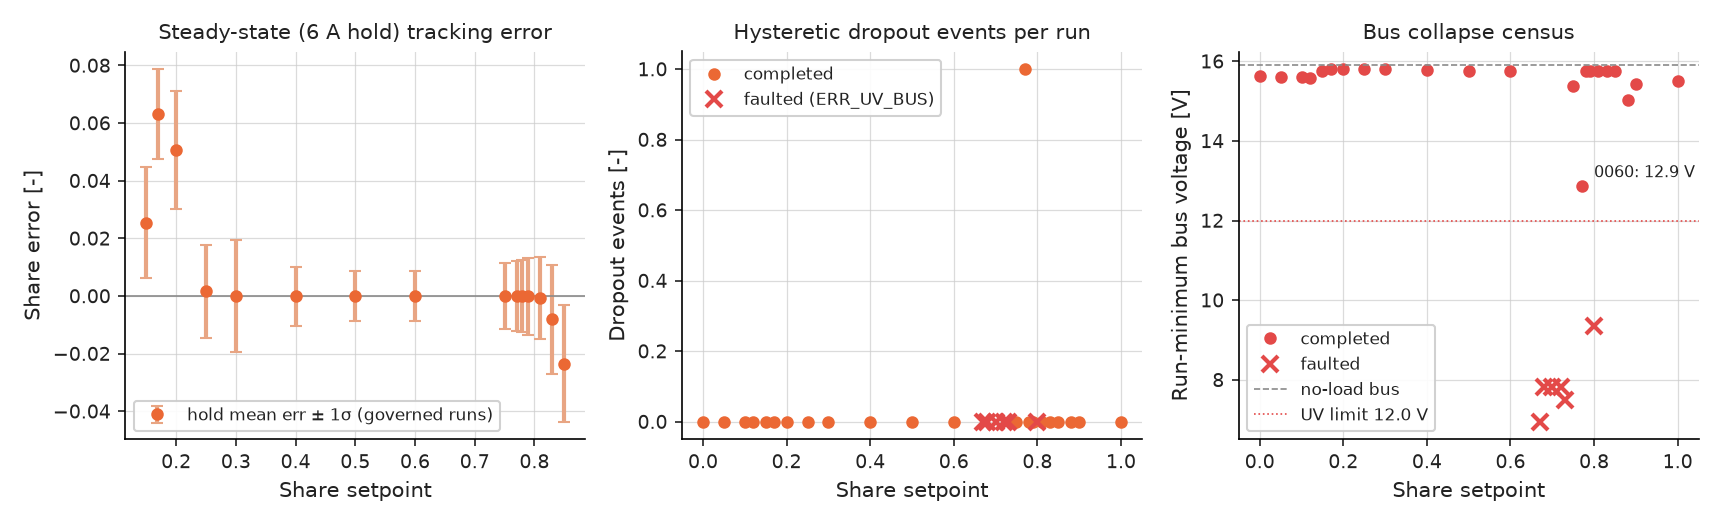
\includegraphics[width=\textwidth]{fig_v4sweep_summary.png}
\caption{Firmware~v4 ladder summary, \code{TP0041}--\code{TP0068}. Left:
hold-window tracking error of the governed (in-band, completed) runs; the
non-zero means at 0.15--0.20 and 0.83--0.85 are the raised governor floor
clipping at hold, not loop error. Center: hysteretic dropout events --- zero
everywhere, including the six faulted runs, whose relay cycle never co-conducts
and is therefore invisible to a minority-dropout counter. Right: run-minimum bus
voltage; crosses mark the six \code{ERR\_UV\_BUS} latches, and \code{TP0060} is
the surviving near-miss at 12.9\,V.}
\label{fig:v4summary}
\end{figure}

\subsection{A new failure mode: the source-commutation relay cycle}
\label{sec:relay}

Six runs at fuel-cell-heavy setpoints latched \code{ERR\_UV\_BUS}
(Table~\ref{tab:v4faults}), at setpoints that were clean on firmware~v3.
The mechanism is not the minority-channel dropout cycle: the channels
\emph{alternate exclusive ownership} of the bus. Figure~\ref{fig:tp0053relay}
shows \code{TP0053}. One channel conducts alone for tens of milliseconds while
its droop gain climbs; at a reproducible commanded-ratio threshold, ownership
commutates through a 7--12\,ms window in which \emph{both} channels read zero and
the $\approx$1\,mF motor node discharges unopposed; the other channel then
reconnects with a 2--3\,A burst and the pattern mirrors. The full period is
16--20\,Hz. Because co-conduction never occurs, the hysteretic minority-dropout
counter of Figure~\ref{fig:v4summary} reads zero for these runs --- the counter
discriminates the two topologies.

\begin{table}[H]
\centering
\small
\caption{The six \code{ERR\_UV\_BUS} runs. ``Relay onset'' is the first
exclusive-conduction handoff; ``first $<$12\,V'' is the first bus sample under
the fault limit; ``latch delay'' is from that sample to the end of the log.}
\label{tab:v4faults}
\begin{tabular}{llrrrr}
\toprule
Run & $r^\ast$ & Relay onset [s] & First $<$12\,V [s] & $V_\mathrm{bus}$ min [V] & Latch delay [ms] \\
\midrule
\code{TP0055} & 0.67 & 3.48 & 3.96 & 6.95 & 1029 \\
\code{TP0054} & 0.68 & 3.30 & 3.88 & 7.83 & 1007 \\
\code{TP0053} & 0.70 & 3.54 & 3.93 & 7.82 & 1320 \\
\code{TP0056} & 0.72 & 3.47 & 3.88 & 7.83 & 1164 \\
\code{TP0057} & 0.73 & 3.39 & 3.87 & 7.49 & 1289 \\
\code{TP0059} & 0.80 & 4.08 & 4.38 & 9.35 & 413 \\
\bottomrule
\end{tabular}
\end{table}

\begin{figure}[H]
\centering
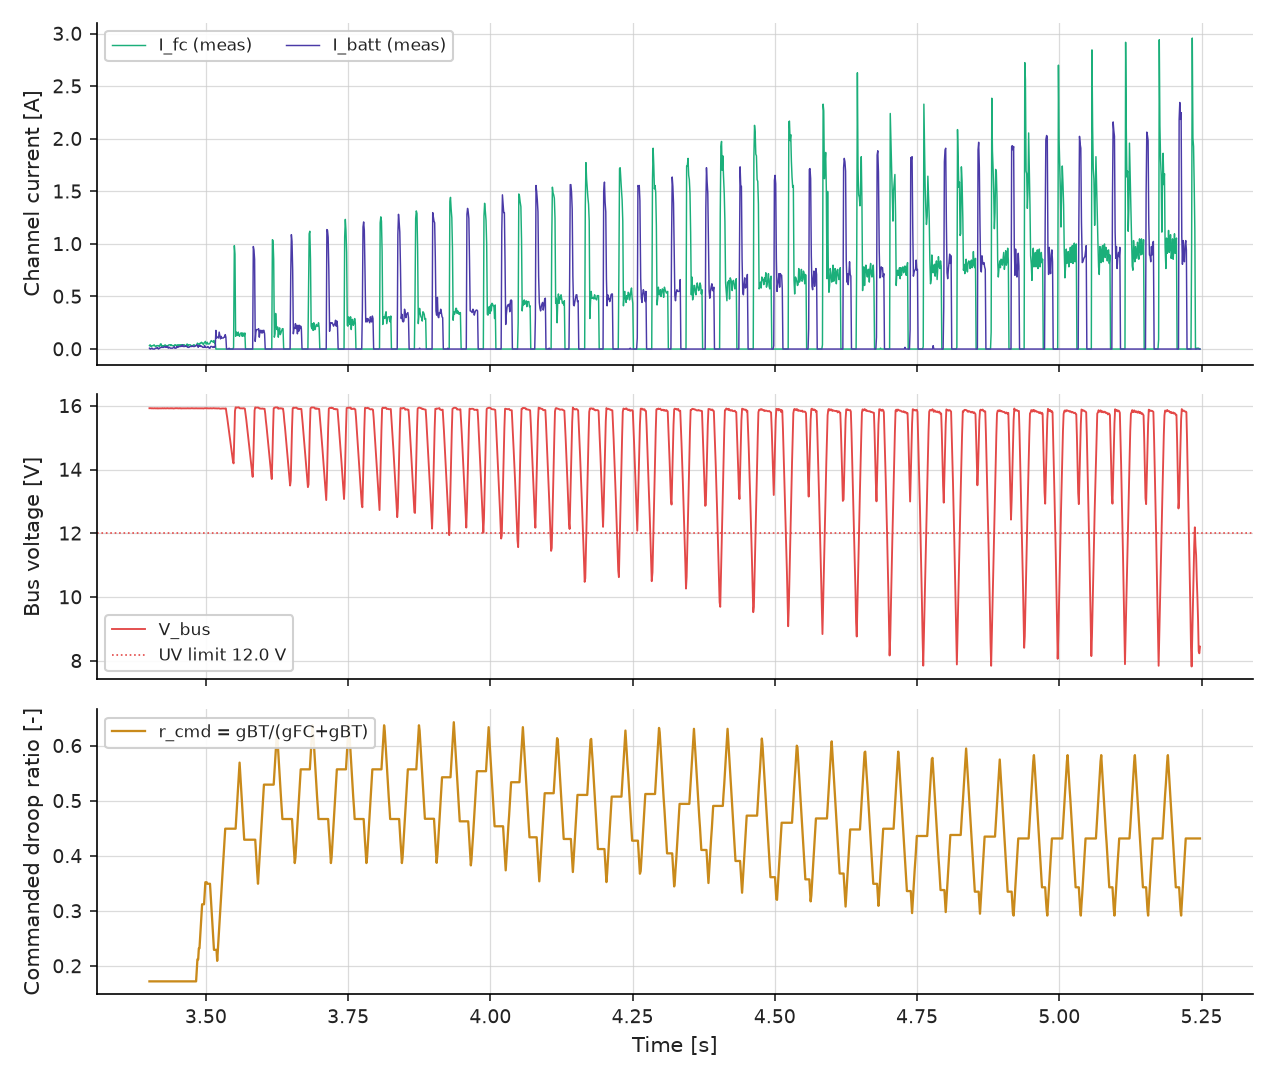
\includegraphics[width=0.95\textwidth]{fig_tp0053_relay.png}
\caption{\code{TP0053} ($r^\ast=0.70$): the source-commutation relay cycle.
Top: FC and BT alternate exclusive conduction with 2--3\,A reconnect bursts;
co-conduction never occurs. Middle: each both-channels-off handoff window
discharges the motor node, and the troughs walk monotonically down through the
12\,V fault limit as the load ramp steepens the discharge slope. Bottom: the
commanded droop ratio sawtooths between reproducible commutation thresholds at
the slew-limited rate.}
\label{fig:tp0053relay}
\end{figure}

The entry condition is the governor's own fallback. The share loop wakes at
\code{SHARE\_I\_TOT\_MIN\_A} $=0.075$\,A of total current, and the governor
filter --- reset at profile start --- reads well under the 0.60\,A collapse
threshold, so the effective setpoint is 0.5 in every run at wake. At
0.1--0.5\,A of total current, however, a 0.5 split commands 0.05--0.25\,A per
channel --- \emph{below the 0.30\,A floor the governor exists to enforce} ---
against a droop authority of order 20\,mV, which the channel offset voltage
$\Delta V_0$ exceeds. The split is physically unachievable; the controller
saturates at the slew limit and commutates ownership instead of sharing. The
collapse-to-0.5 fallback therefore commands, throughout the window
$0.075 \leq I_\mathrm{tot} \leq 0.60$\,A, exactly the class of infeasible split
whose avoidance is its purpose.

Why firmware~v3 survived the identical setpoints and profile
(\code{TP0029}--\code{TP0033}: zero events) is not settled. The leading
candidate --- \textbf{unconfirmed} --- is the floor increase itself: on the
fuel-cell-heavy side the raised clip demands 50\,\% more minority current
through the whole escape window (at 0.6\,A filtered total, v3 asks the battery
channel for 0.20\,A, v4 for 0.30\,A), which plausibly explains failure to
escape rather than entry. The asymmetry fits: below $r^\ast=0.5$ the collapse
pulls \emph{toward} the fuel-cell-dominant natural topology and all twelve runs
are clean; the boundary within 0.67--0.81 is sharp but not monotonic
(0.75 and 0.77--0.79 survive between faults at 0.73 and 0.80).
\code{TP0060} ($r^\ast=0.77$) is the diagnostic near-miss: it entered the same
relay at $t=3.68$\,s, ratcheted the bus to 12.88\,V --- 0.88\,V above the
limit --- and escaped cleanly at $t=3.92$\,s once total current reached
$\approx$0.25\,A and droop authority overcame $\Delta V_0$, then tracked its
setpoint without incident for the remaining eleven seconds.

\subsection{The undervoltage fault: correct, and too slow for this waveform}

The new fault behaved exactly as specified in all six events: raw
\code{fault\_flags} indication from the first sub-12\,V sample, one clean latch,
no re-arm, \code{close\_reason=fault} with \code{error\_code=9}. The
specification, however, is mistuned for the relay waveform. The cycle holds the
bus under 12\,V for $\approx$9\,ms and above it for $\approx$51\,ms; each
excursion falls just short of the 10\,ms persistence window, and each 51\,ms gap
exceeds the 5\,ms gap guard and resets the accumulator. The runs therefore
endured 1.0--1.3\,s and up to 24 excursions --- to minima of 6.95\,V --- before a
window finally bridged (\code{TP0059} latched in 413\,ms only because its final
excursion never recovered). The filter also proved its other edge:
\code{WP0069} logged a genuine transient (13 both-channel dropout events over
208\,ms, bus to 11.56\,V, longest under-run 2.3\,ms) that set the raw flag on
seven samples and correctly did \emph{not} latch, and the run completed.
Recommended retuning: accumulate under-limit dwell in a leaky integrator (or
extend the gap guard beyond one relay period $\approx$60\,ms) so a repeating
sub-limit waveform latches within a few cycles, while a single 2\,ms notch still
passes.

\subsection{\code{W}-profile boundary: the floor law fails at higher load, and
the MCU dies upstream of the bus}
\label{sec:wpv4}

The five \code{W} runs ladder the clip bound $b$: 0.35, 0.30, and 0.25 complete
cleanly; 0.20 and 0.22 truncate mid-run with no trailer --- both at the same
profile boundary, 18.470 and 18.477\,s, where region~R6 (share setpoint at the
$1-b$ bound, 6\,A command) hands off to R7. Figure~\ref{fig:wpboundary} shows
the failure boundary directly: at $b=0.25$ (setpoint 0.75, commanded minority
0.399\,A) region R6 is a crisp step; at $b=0.22$ (setpoint 0.78, commanded
minority 0.381\,A) the battery channel chops at 18.7\,Hz for the full region.
The clean/cycling bracket $(0.381, 0.399)$\,A sits \emph{above} the 0.30\,A
floor --- and above the firmware-v3 bracket $(0.245, 0.29)$\,A measured at
$\approx$1.6\,A total. A single constant-current floor cannot satisfy both
datasets. Either the floor scales with total current (a ripple-clearance
reading) or the true limit is a minority \emph{fraction} of approximately
0.22--0.25, in which case the usable droop band is nearer $[0.25, 0.75]$ than
$[0.15, 0.85]$. The two readings are inseparable in this data --- total current
spanned only 1.59--1.73\,A across the boundary --- and a two-axis sweep
($I_\mathrm{max}$ at fixed setpoint, setpoint at fixed $I_\mathrm{max}$) is the
highest-value next bench session.

\begin{figure}[H]
\centering
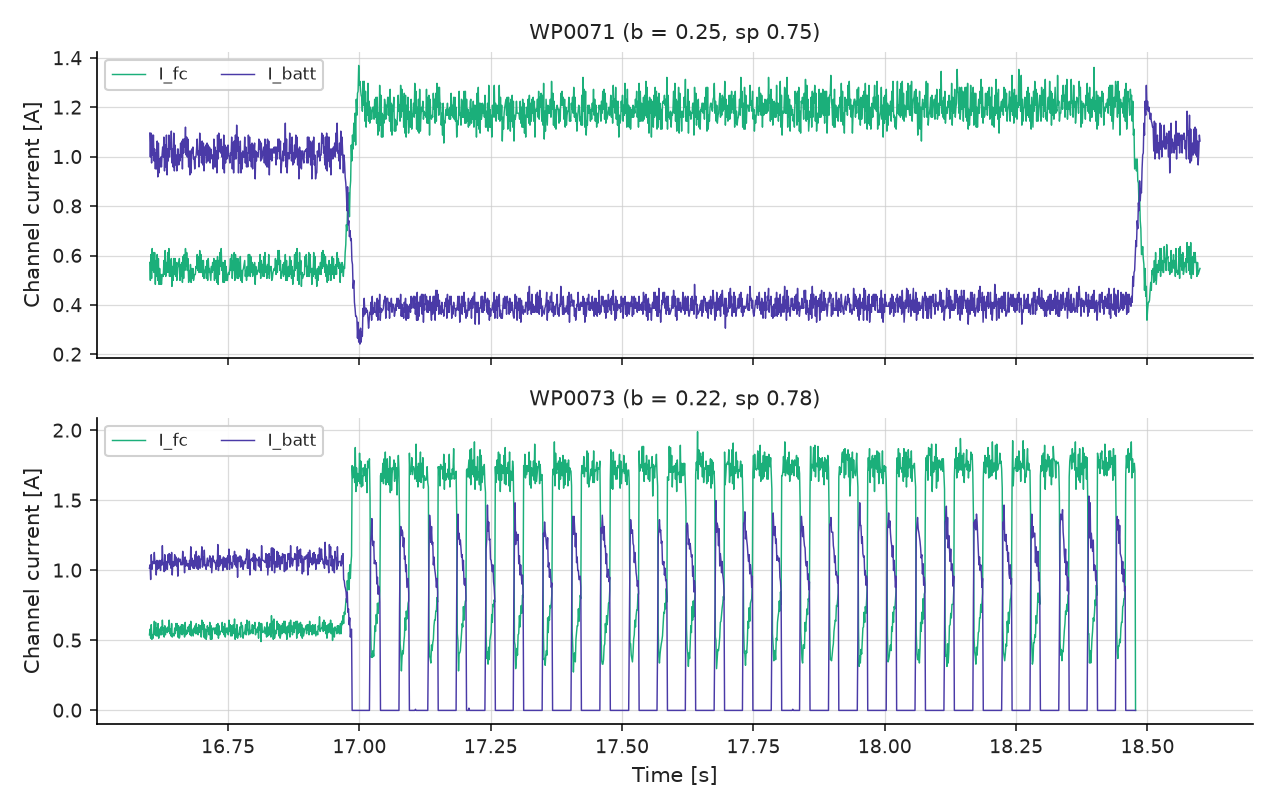
\includegraphics[width=0.95\textwidth]{fig_wp_boundary.png}
\caption{The floor-law failure boundary in region R6 of the \code{W} profile
(share setpoint steps to $1-b$ at 6\,A command). Top: \code{WP0071}
($b=0.25$, commanded minority 0.399\,A) --- a clean step and steady
co-conduction. Bottom: \code{WP0073} ($b=0.22$, commanded minority 0.381\,A) ---
an 18.7\,Hz single-channel dropout cycle for the entire region; the log
truncates at 18.48\,s.}
\label{fig:wpboundary}
\end{figure}

The limit cycle itself (Figure~\ref{fig:wp0072cycle}) is the classical
minority-dropout topology of Section~\ref{sec:limitcycle}, with one new
observation: its frequency is set by the slew limiter. The commanded ratio
traverses a 0.48-wide triangle at 0.02 per tick --- 27.9\,ms per leg, a 55.8\,ms
period --- matching the observed 53.9\,ms. The firmware-v2 slew limit converts
the original bang-bang instability into a bounded triangle oscillation; it does
not suppress it.

\begin{figure}[H]
\centering
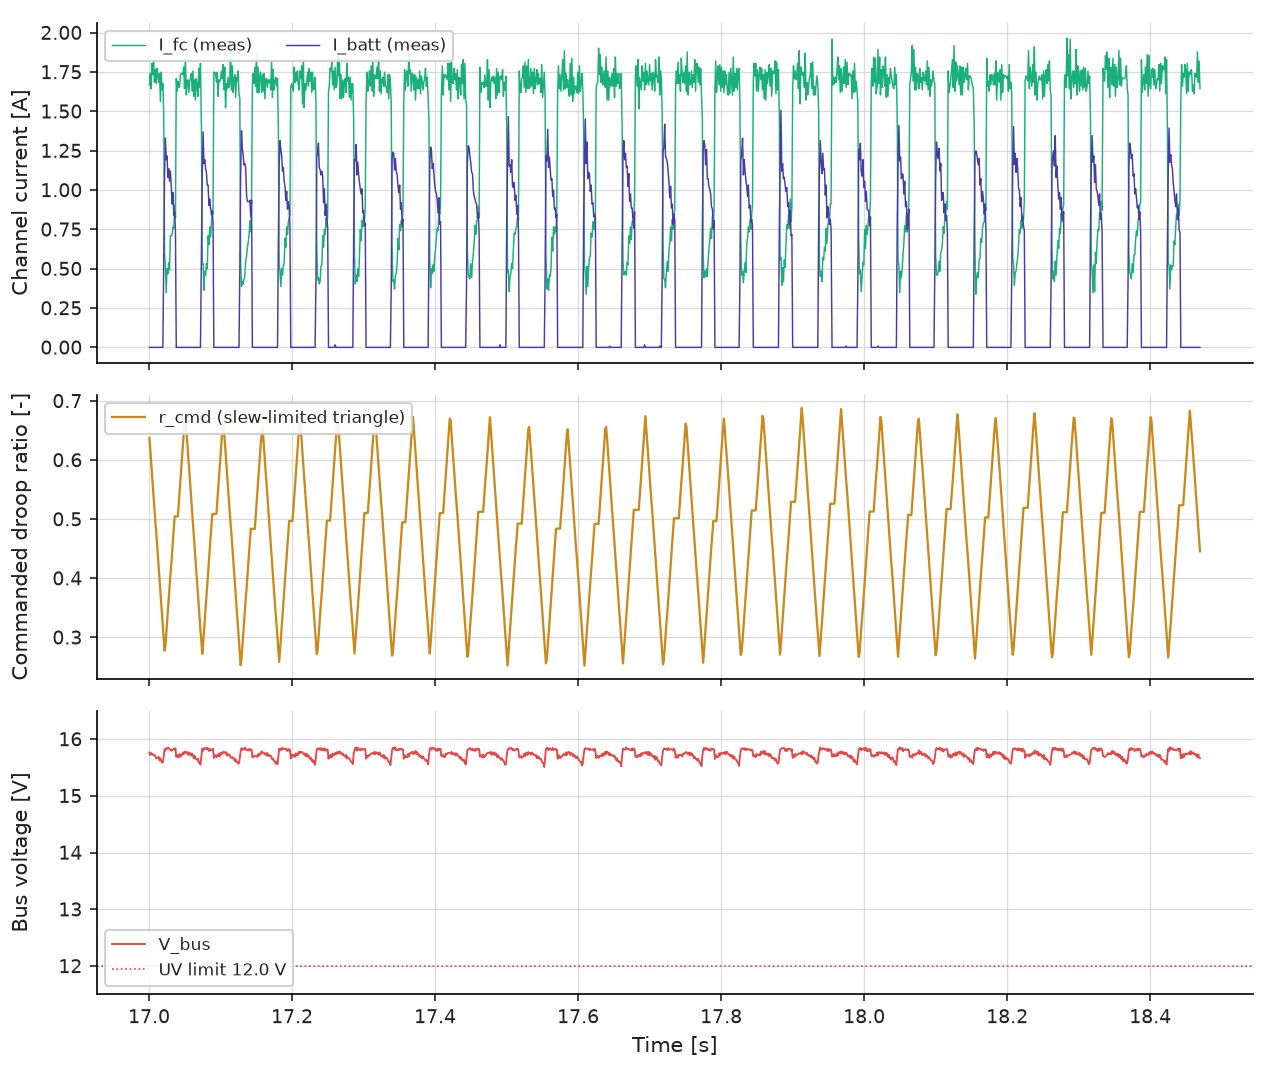
\includegraphics[width=0.95\textwidth]{fig_wp0072_cycle.png}
\caption{\code{WP0072} ($b=0.20$), final 1.5\,s before truncation. Top: the
battery channel drops and reconnects at 18.7\,Hz while the fuel-cell channel
absorbs the full load. Middle: the commanded droop ratio is a slew-rate-limited
triangle --- the 0.02-per-tick limit sets the 54\,ms period. Bottom: the bus
never leaves regulation (ripple 0.35\,V, minimum 15.51\,V); the MCU brownout
that truncates the log is invisible on every logged channel.}
\label{fig:wp0072cycle}
\end{figure}

The truncations themselves are the campaign's most consequential result. In both
runs the bus was in regulation at 15.7\,V at the final record, \code{fault\_flags}
was zero throughout, the sample interval was nominal to the last sample, and the
gains were still slewing --- no fault latched, and no electrical precursor
appears on any logged channel. The MCU (board-powered through the LM1084 from
the battery source rail) browned out from an \emph{upstream} collapse that the
bus-referenced undervoltage fault is structurally incapable of observing. The
reboot is confirmed by \code{start\_millis}: \code{WP0073} began 19.6\,s after
\code{WP0072}'s power cycle. Both deaths within 12\,ms of the same region
boundary --- with the reconnect burst still 8--15\,ms away --- implicate the
setpoint step itself, through a channel this log does not instrument. Two
actions follow: instrument the source rails (the \code{BT\_VOLTAGE} ADC input
exists and is not logged) and consider a source-rail undervoltage fault; and
scope \code{VBT} and the LM1084 input across an R6$\to$R7 step before further
$b \leq 0.22$ runs.

\section{Third validation sweep (firmware v5)}
\label{sec:v5}

\subsection{Mitigation set and sweep design}

Firmware~v5 implements the three actions recommended in
Section~\ref{sec:conclusions} items~9, 11, and~12. First, the governor's
collapse-to-0.5 fallback is deleted. The loop is now bimodal on the filtered
total current: closed-loop control engages above 0.60\,A and releases below
0.55\,A. Below the threshold the loop runs \emph{open-loop}: if closed-loop
control has not yet run, the raw in-band setpoint is fed forward through the
0.02-per-tick slew limiter; otherwise the last applied ratio is held frozen.
Out-of-band setpoints are never actuated by the feedforward. Second, the
undervoltage persistence window is replaced by a \emph{leaky dwell integrator}:
time under 12.0\,V accumulates at full rate (capped at 5\,ms per tick), time
above it leaks off at 5\,\%, and 20\,ms of net dwell latches the fault. Third,
the log format now records the four source-side rails (\code{FC\_VOLTAGE},
\code{BT\_VOLTAGE}, \code{CHG\_VOLTAGE}, \code{RGN\_VOLTAGE}) at the full 1\,kHz
rate, closing the instrumentation gap identified after the firmware~v4
brownouts.

The campaign comprises a 21-point trapezoid ladder
(\code{TP0074}--\code{TP0094}, identical \code{T 6 3 1} profile) run as two
automated batches within one boot --- setpoints 0 to 0.50 ascending, then 0.90
down to 0.60 --- and seven \code{W} combined profiles
(\code{WP0095}--\code{WP0101}, $I_\mathrm{max}=6$\,A) at share-clip bounds
$b = 0.30$, 0.20, 0.15 ($\times3$), and 0 ($\times2$). The bound $b$ is not
recorded in the log header; it is recovered here from the clipped setpoint
itself, $b = 1 - \max(\code{share\_sp})$, a method that reproduces both
operator-confirmed labels. Every trapezoid run completed cleanly. Five of the
seven \code{W} runs failed at the same profile event
(Section~\ref{sec:r6}); each failure forced a power cycle, so
\code{WP0097}--\code{WP0101} are single-run or short fresh-boot sessions.

\subsection{The trapezoid ladder is clean end to end}

Figure~\ref{fig:v5summary} summarizes the ladder: 21 of 21 runs complete, zero
fault flags in every sample, and no bus sample below 14.89\,V anywhere in the
campaign. The firmware~v4 relay region is closed. Table~\ref{tab:v5relay}
compares the four relay-cycle setpoints directly.

\begin{table}[H]
\centering
\caption{The firmware~v4 relay-cycle setpoints, re-run on firmware~v5.
Firmware~v4 columns aggregate \code{TP0053}--\code{TP0057} and \code{TP0059};
firmware~v5 columns are \code{TP0090}--\code{TP0093}.}
\label{tab:v5relay}
\begin{tabular}{lcc}
\toprule
Metric & firmware~v4 & firmware~v5 \\
\midrule
Faults & \code{ERR\_UV\_BUS}, every run & none \\
Bus minimum & 7--9\,V & 15.71--15.73\,V \\
Exclusive-conduction fraction & $\approx$100\,\% & 0\,\% \\
Both-channels-off gaps in hold & 7--12\,ms, repeating & none $\geq$3\,ms \\
Commutation signature & 16--20\,Hz & no 14--24\,Hz spectral peak \\
Hold-window share error (mean) & undefined (commutating) & $\leq 3\times10^{-5}$ \\
\bottomrule
\end{tabular}
\end{table}

Tracking bias in the 6\,A hold window is below $10^{-3}$ at every in-band
setpoint from 0.18 to 0.82. The two band-edge runs show the governor clip, not
a tracking failure: at $r^\ast=0.15$ the floor raises the effective setpoint to
0.169 and the measured share lands $+1.5\times10^{-3}$ from it
($+0.020$ from the raw value); at $r^\ast=0.85$ the clip is active in the other
direction ($-0.013$ from the raw value). The five out-of-band runs
($r^\ast \in \{0, 0.10, 0.12, 0.88, 0.90\}$) latch a hard single-channel cut:
the starved channel's measured current is exactly zero for the whole run, the
controller stays frozen, and the isolated dropout-counter events in
Figure~\ref{fig:v5summary} are threshold-crossing artifacts at the ramp edges,
not cycling. The spectral check is negative everywhere: over every hold window
the 14--24\,Hz band carries 4--6\,\% of the residual energy with no peak.

\begin{figure}[H]
\centering
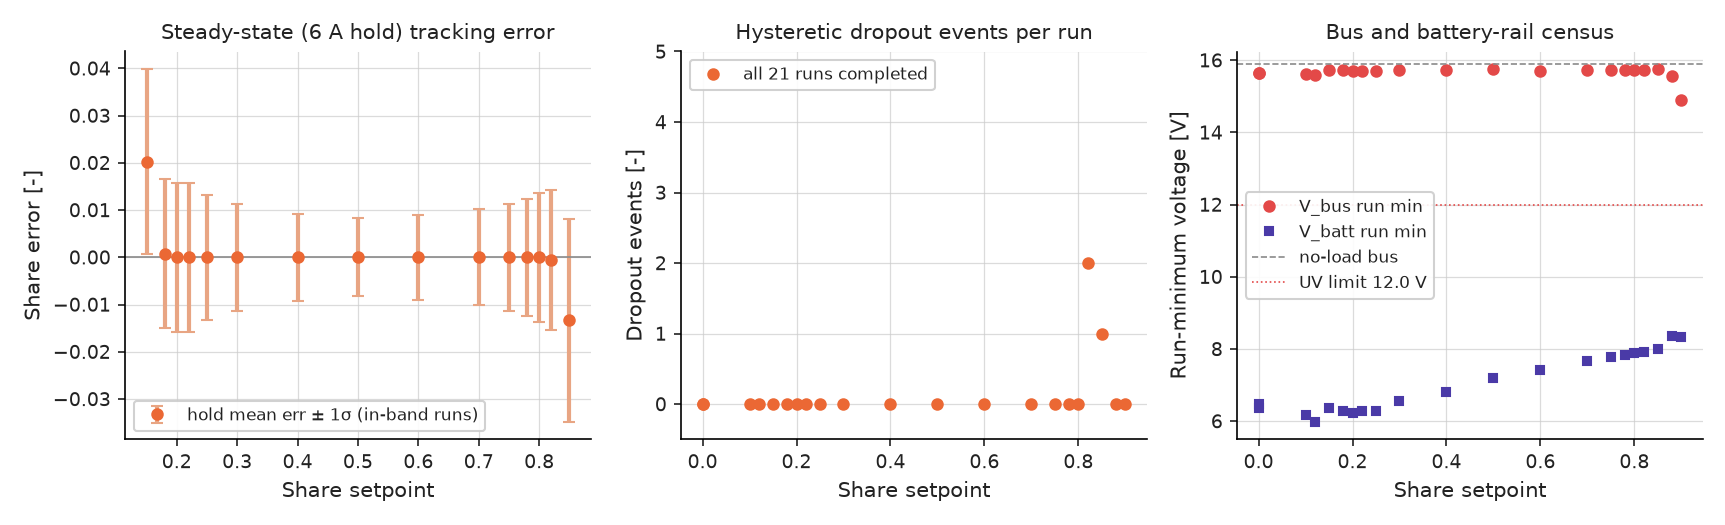
\includegraphics[width=\textwidth]{fig_v5sweep_summary.png}
\caption{Firmware~v5 trapezoid ladder (\code{TP0074}--\code{TP0094}). Left:
hold-window tracking error versus the raw setpoint; the two outliers at 0.15
and 0.85 are the governor clip acting as designed. Center: dropout events; the
two nonzero counts (1 at 0.85, 2 at 0.82) are ramp-edge threshold crossings,
with zero events inside any hold window. Right: run-minimum bus and
battery-rail voltages; the battery rail dips lowest where the battery is the
sole source (setpoints $\leq0.12$), reaching 5.98\,V at $r^\ast=0.12$.}
\label{fig:v5summary}
\end{figure}

The governor's new machinery is directly observable in the logs. The open-loop
feedforward appears as an exact 0.02-per-tick staircase that lands on the raw
setpoint to four decimal places; each run inherits its predecessor's final
ratio as the staircase seed, confirming that the slew tracker survives the
per-profile state reset as designed. Every in-band run shows exactly two mode
edges --- closed-loop entry at 0.60--0.73\,A of total current on the ramp-up,
release to hold at 0.40--0.52\,A on the ramp-down --- with zero chatter, and
the held ratio is frozen to numerical exactness for the remaining 2.5\,s of
every run.

Three residual observations temper the pass. First, the open-loop feedforward
applies the \emph{raw} setpoint while closed-loop control applies the
\emph{floor-clipped} setpoint, so the handover at 0.60\,A commands a
discontinuous step; at $r^\ast=0.15$ the effective setpoint jumps from 0.15 to
0.50 and roughly 0.25\,A commutates between the sources over
$\approx$17\,ticks. No run showed any consequence, but the step is unnecessary
--- the clip can be applied to the feedforward as well. Second, the floor
bounds the commanded minority current only: measured minority current dips to
0.193\,A at $r^\ast=0.15$ and 0.20--0.24\,A at 0.82--0.85, inside the old
cycling bracket, without igniting anything. Third, the battery rail is the
soft one ($\approx$0.9--1.0\,V/A source slope, versus $\approx$0.28\,V/A for
the fuel-cell side), and battery-sole-source runs push it hardest:
$r^\ast=0.12$ reached 5.98\,V and the $r^\ast=0$ repeat spent 3.6\,s below
7.0\,V. These runs are the brownout-risk case for any higher-current session.

\subsection{The R6 share-bound excursion is the \code{W}-profile failure
generator}
\label{sec:r6}

All five \code{W} failures occur at the same profile event: entry into region
R6 at $t\approx17.0$\,s, where the profile steps the share command to 1.00
(clipped to $1-b$) while the motor axis remains at the full 6\,A command ---
the only region that combines peak load with an extreme share. Nothing about
the current command changes at the boundary; the share step alone is lethal,
and its severity is ordered monotonically by the clipped target
(Table~\ref{tab:v5w}).

\begin{table}[H]
\centering
\caption{\code{W}-profile outcomes, firmware~v5, ordered by the R6 clipped
setpoint $1-b$. Total current entering R6 is 1.8--2.0\,A in every run. ``Time
in R6'' is from region entry to the last record.}
\label{tab:v5w}
\begin{tabular}{llllll}
\toprule
Run & $b$ & R6 target & R6 behaviour & Outcome & Time in R6 \\
\midrule
\code{WP0095} & 0.30 & 0.70 & converges, minority 0.54\,A & complete & (full 1.5\,s) \\
\code{WP0100} & 0.15 & 0.85 & 18.8\,Hz dropout cycle, 28 episodes & complete & (full 1.5\,s) \\
\code{WP0096} & 0.20 & 0.80 & dropout cycle, 4 episodes & truncation & 197\,ms \\
\code{WP0098} & 0.15 & 0.85 & dropout cycle, 2 episodes & truncation & 86\,ms \\
\code{WP0099} & 0.15 & 0.85 & dropout cycle, 5 episodes & truncation & 254\,ms \\
\code{WP0097} & 0 & 1.00 & setpoint latch cuts BT under load & \code{ERR\_UV\_BUS} & 43\,ms \\
\code{WP0101} & 0 & 1.00 & setpoint latch cuts BT under load & \code{ERR\_UV\_BUS} & 39\,ms \\
\bottomrule
\end{tabular}
\end{table}

\paragraph{Target 0.70: feasible.} \code{WP0095} converges to $r\approx0.68$
with the battery channel at 0.54--0.68\,A and completes the region with a flat
bus. No incipient cycling is visible at any sensitivity.

\paragraph{Targets 0.80--0.85: the firmware~v4 dropout cycle, in band.} The
setpoint is inside $[0.15, 0.85]$, so no latch fires and the closed loop stays
live. The equilibrium it is asked for is infeasible, and the loop limit-cycles:
the battery channel stops conducting, the controller walks the ratio back down
at the slew ceiling, the channel reconnects, and the cycle repeats at 18.8\,Hz
--- the period set by the 0.02-per-tick limit walking the ratio triangle
(Figure~\ref{fig:wp0100r6}). This is the firmware~v4 pre-brownout mode, not the
relay cycle: the fuel-cell channel conducts continuously and there are no
both-off gaps. The governor is structurally inert here --- at 2\,A total the
floor clips only outside $[0.15, 0.85]$, so targets 0.80 and 0.85 pass through
unmodified --- and the channel drops out at a \emph{commanded} minority current
of 0.55--1.04\,A, two to three times the 0.30\,A floor.

\begin{figure}[H]
\centering
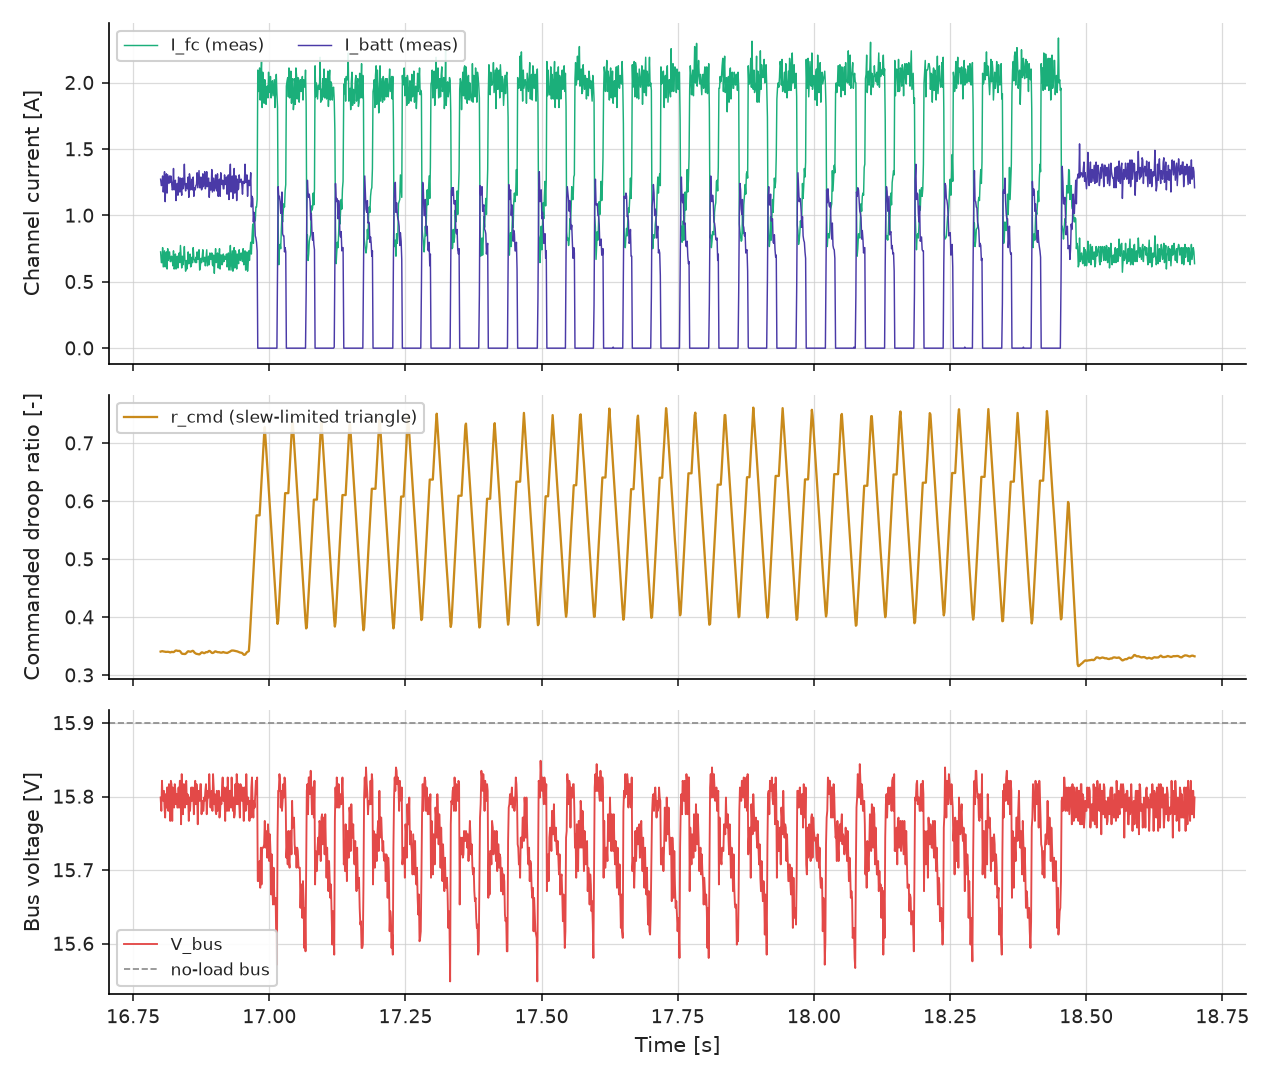
\includegraphics[width=0.95\textwidth]{fig_wp0100_r6.png}
\caption{\code{WP0100} ($b=0.15$), region R6. Top: the battery channel drops
out and reconnects 28 times at 18.8\,Hz while the fuel-cell channel carries the
full $\approx$2\,A. Middle: the commanded droop ratio is the slew-limited
triangle between $\approx$0.39 and $\approx$0.75. Bottom: the bus notches by
$\approx$0.25\,V per episode but never approaches the 12\,V limit. The cycle
self-terminates the instant R7 steps the setpoint back to 0.35.}
\label{fig:wp0100r6}
\end{figure}

Whether a run at target 0.80--0.85 survives is decided not by the cycle itself
but by the fuel-cell source. During each battery-off half-cycle the fuel-cell
input carries the whole load, and the source exhibits a hard knee at
$\approx$2.1\,A: \code{WP0100} ran 28 consecutive solo episodes at
1.96--2.08\,A with the rail flat at 7.8\,V, while \code{WP0096},
\code{WP0098}, and \code{WP0099} drew 2.11--2.19\,A and the rail collapsed
within two to five episodes (Figure~\ref{fig:fcknee}). Roughly 0.1\,A of motor
load separates the clean run from the three deaths. Once the rail falls, the
boost demands more input current to hold the bus --- logged fuel-cell current
spikes reach 6.1\,A as the rail passes below 5\,V --- a positive-feedback
source-collapse runaway. Whether the knee is bench-supply current foldback or
source droop is not distinguishable from the logs.

\begin{figure}[H]
\centering
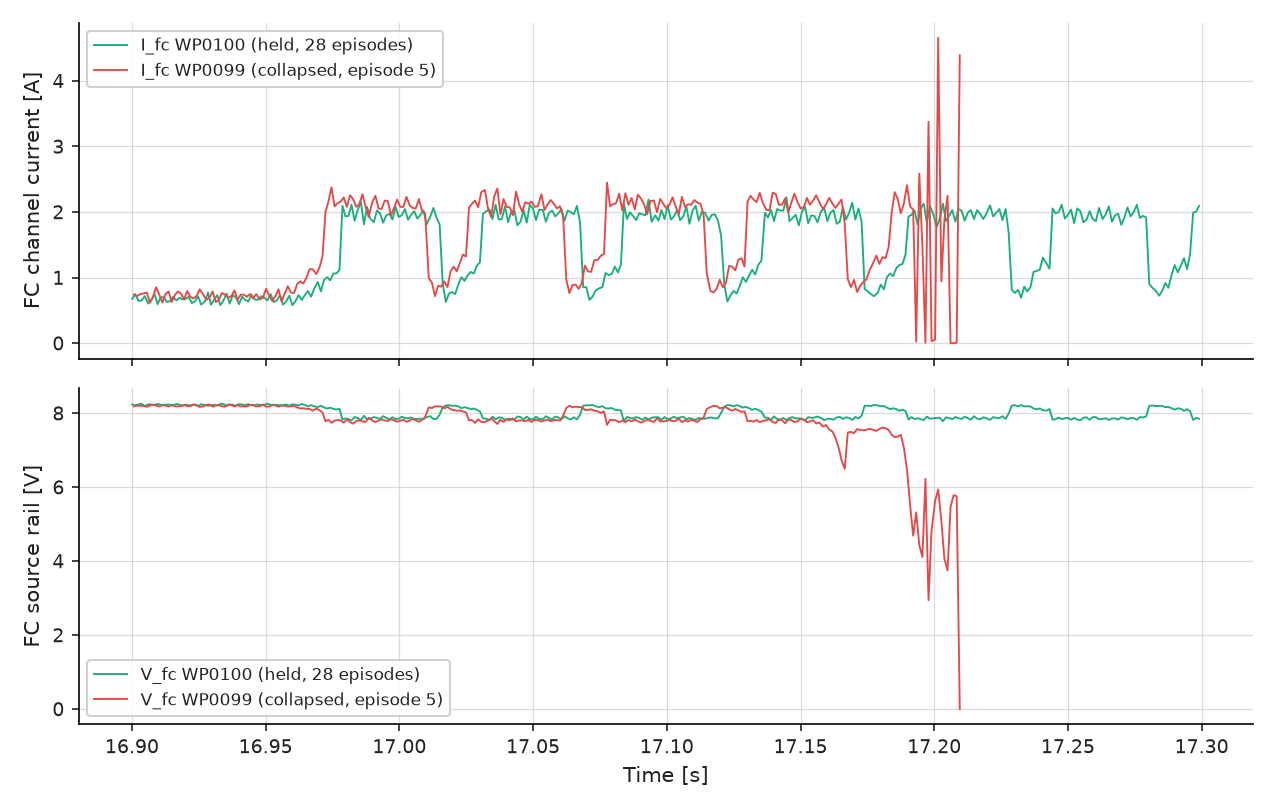
\includegraphics[width=0.95\textwidth]{fig_fc_knee.png}
\caption{The fuel-cell source knee. \code{WP0100} (green) and \code{WP0099}
(red) run the same $b=0.15$ profile; their solo-episode fuel-cell currents
differ by $\approx$0.1\,A. \code{WP0100} holds 7.8\,V through 28 episodes;
\code{WP0099}'s rail collapses on its fifth episode and the input current runs
away.}
\label{fig:fcknee}
\end{figure}

\paragraph{Target 1.00: the setpoint latch becomes the killer.} With $b=0$ the
R6 command exceeds \code{DROOP\_R\_MAX}, and the setpoint-latched cutoff ---
introduced in firmware~v4 to \emph{prevent} switch cycling --- opens the
battery bus switch in one tick under 2\,A of load
(Figure~\ref{fig:wp0101cut}). The battery current steps to zero in one sample
and its rail rebounds to the unloaded 8.4\,V; the fuel-cell source, alone above
its knee, collapses from 7.8\,V through 3.4\,V within 23\,ms; the bus falls out
of regulation and the undervoltage fault latches. Both $b=0$ runs die this way
in under 45\,ms --- the fastest failure in the campaign, and a direct
demonstration that an under-load channel cut is itself a hazardous actuation
when the surviving source cannot carry the total.

\begin{figure}[H]
\centering
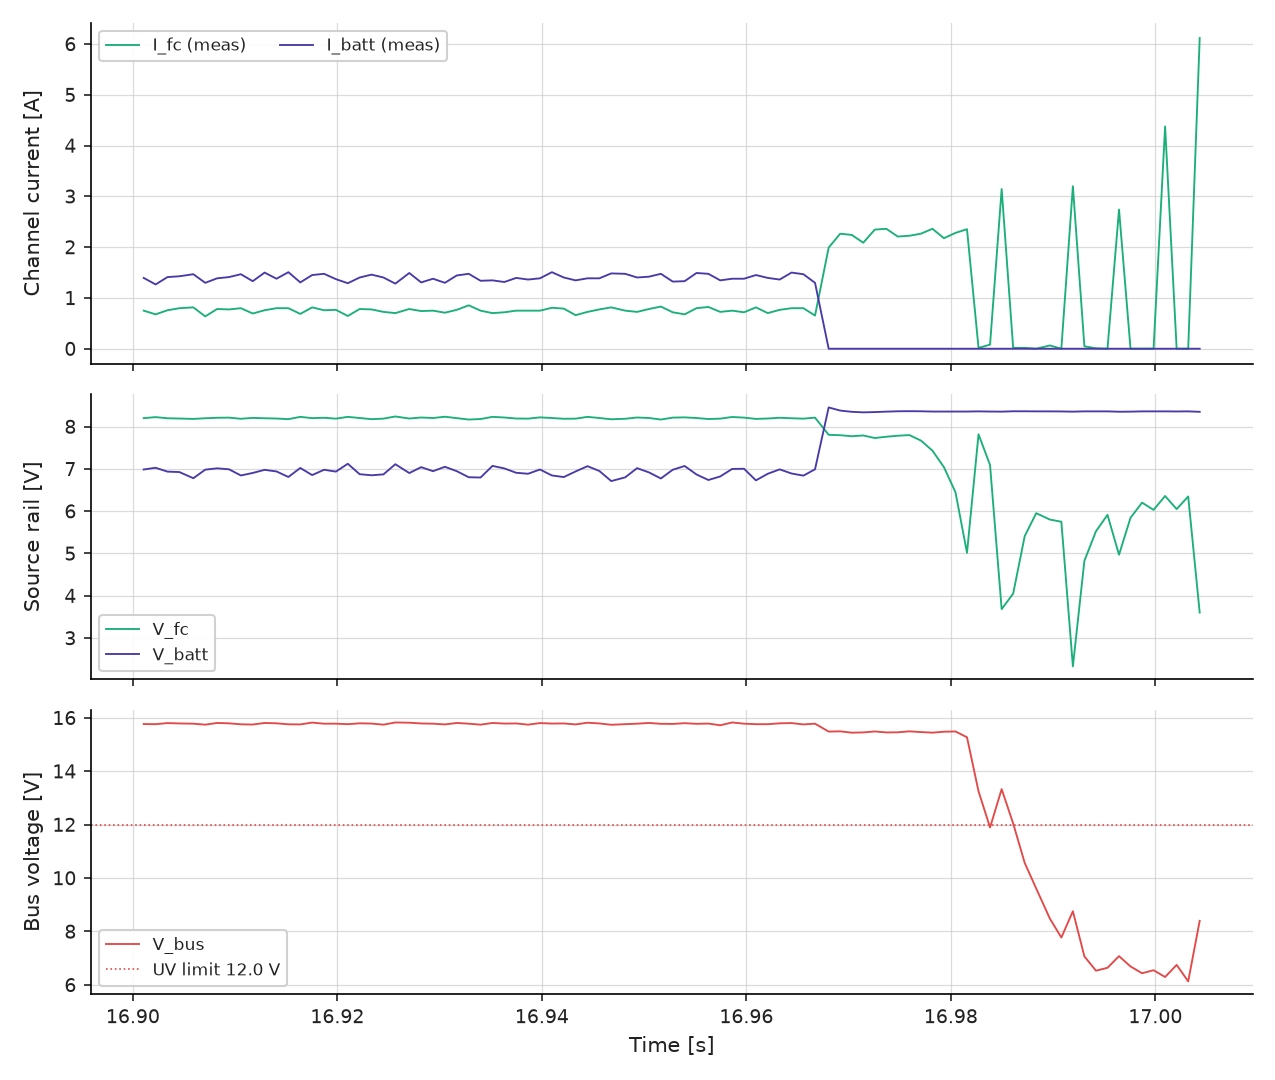
\includegraphics[width=0.95\textwidth]{fig_wp0101_cut.png}
\caption{\code{WP0101} ($b=0$), R6 entry. Top: the setpoint latch cuts the
battery channel in one sample; the fuel-cell channel steps to the full load and
then runs away as its source collapses. Middle: the battery rail rebounds to
its unloaded 8.4\,V --- the battery is healthy and disconnected --- while the
fuel-cell rail falls to 2.3\,V. Bottom: the bus leaves regulation
$\approx$15\,ms after the cut and the dwell-filtered undervoltage fault latches
$\approx$20\,ms later.}
\label{fig:wp0101cut}
\end{figure}

\subsection{The dwell filter is vindicated; the source rail is still
unguarded}

The reworked undervoltage filter performed exactly as designed. In both
\code{ERR\_UV\_BUS} runs the reconstructed dwell integrator crosses 20\,ms
within 18--21\,ms of the first sub-12\,V sample --- against 1.0--1.3\,s of
evasion for the firmware~v4 window on the same class of waveform. No spurious
latch occurred anywhere in the 28-run campaign.

The three truncation runs, however, beat the filter by dying upstream of it.
In \code{WP0096} and \code{WP0098} the bus had spent only 3.4\,ms below
12.0\,V when the MCU stopped; four samples earlier it was in regulation at
15.7\,V. The fuel-cell rail tells the real story the bus cannot: it had been
below 7\,V for $\approx$10\,ms and below 5\,V for $\approx$3\,ms while the bus
still read 15.7\,V. A source-rail undervoltage fault --- the action deferred
from the firmware~v4 round --- would have latched \code{WP0098} roughly 7\,ms
before the bus moved at all. The new rail logging also overturns the working
hypothesis for the MCU stops: the battery rail read 8.37, 8.37, and 7.89\,V
at the three truncation instants --- unloaded in two of them --- so a
battery-rail brownout through the logic regulator is unsupported at the
870\,Hz log rate. The stop mechanism is therefore unconfirmed; either a
sub-millisecond transient invisible to the log, or a path other than the
battery rail, stops the processor. Oscilloscope captures 13 and 14 (taken
under the \code{WP0101} condition) corroborate the logged chronology --- the
battery current envelope collapses in one step, the battery rail recovers
upward to 8.4\,V, and the motor node decays 15.9 to 8.4\,V over 19.4\,ms ---
and capture 14 additionally resolves what the log cannot: late in the decay,
as the motor node falls through the battery-rail level, the battery rail dips
$\approx$0.9 division below its 8.4\,V baseline at 5\,V per division ---
to $\approx$4--5\,V --- for under a millisecond, within $\approx$2\,ms of a
full-scale battery-current spike. A battery-rail transient of that depth is
below the LM1084 dropout for the logic rail, and its sub-millisecond width is
invisible at the 870\,Hz log rate --- which reconciles the healthy logged
battery rail with the observed stops. The inferred mechanism (the collapsing
node reaching the battery rail and drawing reconnect inrush through the source
impedance) is unconfirmed; the settling measurement is a capture on the LM1084
input and output through a truncation event.

\subsection{The floor law, revisited with source-rail data}
\label{sec:floorlaw}

The \code{W} cluster sharpens Section~\ref{sec:conclusions} item~11 into a
structural statement: no absolute-current floor can separate the stable region
from the cycling region, because the boundary is not a current level.
\code{WP0100} dropped out 28 times at a cycle-averaged operating point ---
15.81\,V bus, 0.69\,A battery current --- that is indistinguishable, to within
27\,mV of bus voltage, from the point \code{WP0095} held stably for the full
region. At 0.7\,A the droop offset is only $\approx$0.23\,V, and the measured
channel-offset envelope $\Delta V_0 = \pm0.10$\,V is 40\,\% of that authority,
so conduction is decided by a sub-100\,mV race between the bus and the starved
channel's effective reference. The effect is also one-sided: the fuel-cell
channel held 0.63--0.72\,A as the minority in regions R5 and R7 of every run
with zero dropouts, while the battery channel dropped out at 0.55--1.04\,A.
The asymmetry implicates a channel-specific offset (the $\Delta V_0$ sign, the
battery channel's compensator rework, or layout) rather than a symmetric
conduction floor, and the corrected mitigation should be referred to the
bus-versus-reference margin, not to a current constant. The two-axis sweep
recommended previously should therefore be run per channel direction.

\section{Fourth validation sweep (firmware v6)}
\label{sec:v6}

\subsection{Mitigation set and sweep design}

Firmware~v6 implements five changes derived from Section~\ref{sec:v5}. First, a
\emph{load-aware handoff guard} conditions the setpoint-latched channel cutoff on
the current carried by the channel about to be cut: above
$I_\mathrm{handoff}^{\max}=0.50$\,A the cut is refused and \emph{deferred}, the
closed-loop reference is clipped onto the band edge to migrate the load away, and
the ratio-based cutoff is suppressed on that side. Second, a dwell-filtered
fuel-cell undervoltage fault is added (trip 6.0\,V, arm 7.0\,V, 20\,ms dwell),
placed above the bus undervoltage block so that a simultaneous crossing names the
upstream cause. Third, the closed-loop reference itself is slew-limited at
0.02 per tick, removing the step that the open-loop-to-closed-loop handover
previously applied. Fourth, the \code{W} profile regions R5--R7 are de-rated: the
share-bound excursion R6 now runs at $0.3\,I_\mathrm{max}$ instead of full
command. Fifth, the log header records the per-run profile parameters
$I_\mathrm{max}$ and the share-clip bound $b$ directly.

The campaign comprises a 19-point trapezoid ladder
(\code{TP0102}--\code{TP0120}, \code{T 6 3 1}) and four \code{W} combined
profiles (\code{WP0121}--\code{WP0124}). The entire set is a single boot: the
absolute log timestamps run monotonically from 66\,s to 1340\,s with no reset,
in two automated batches separated by a 508\,s idle gap. The header change
removes the inference step used in Section~\ref{sec:v5}: $b$ and
$I_\mathrm{max}$ are now read directly, giving $b=0.30$, 0.20, 0.00, 0.00 and
$I_\mathrm{max}=6$, 6, 6, \textbf{8}\,A for the four \code{W} runs. The last of
these is the first run of the campaign at an $I_\mathrm{max}$ above 6\,A.

\subsection{The targeted fixes all hold}

Every firmware-v6 mechanism performed as specified, verified directly in the
logged data.

\begin{itemize}
\item \textbf{Reference slew.} The largest sample-to-sample step in the commanded
droop ratio across all 23 runs is 0.0200, exactly the limit, with no exceedance
anywhere. The handover step is eliminated.
\item \textbf{Governor floor.} Measured hold share equals
$\max(r^\ast, 0.30\,\mathrm{A}/I_\mathrm{tot})$ to within $10^{-3}$ at every
setpoint. Figure~\ref{fig:v6summary} (left) shows that the apparent standing bias
at $r^\ast=0.15$ and 0.17 is entirely this clip: referred to the governed
setpoint the error collapses to $\le2\times10^{-3}$.
\item \textbf{Bimodal governor.} Exactly two mode transitions per governed run,
entry at 0.65--0.75\,A and release at 0.40--0.50\,A of instantaneous total, zero
chattering, and no stranded hold state.
\item \textbf{Fuel-cell undervoltage fault.} Armed throughout its first flight
with zero false trips, including in the six runs where the fuel-cell channel is
latched off the bus.
\end{itemize}

\code{fault\_flags} is zero in every sample of all 23 runs, and the census of
total source dropouts --- both channels dark while the pair was conducting
immediately before --- returns \textbf{one event in nineteen ladder runs}. That
event is \code{TP0115}, and it is the subject of Section~\ref{sec:v6edge}.

\begin{figure}[H]
\centering
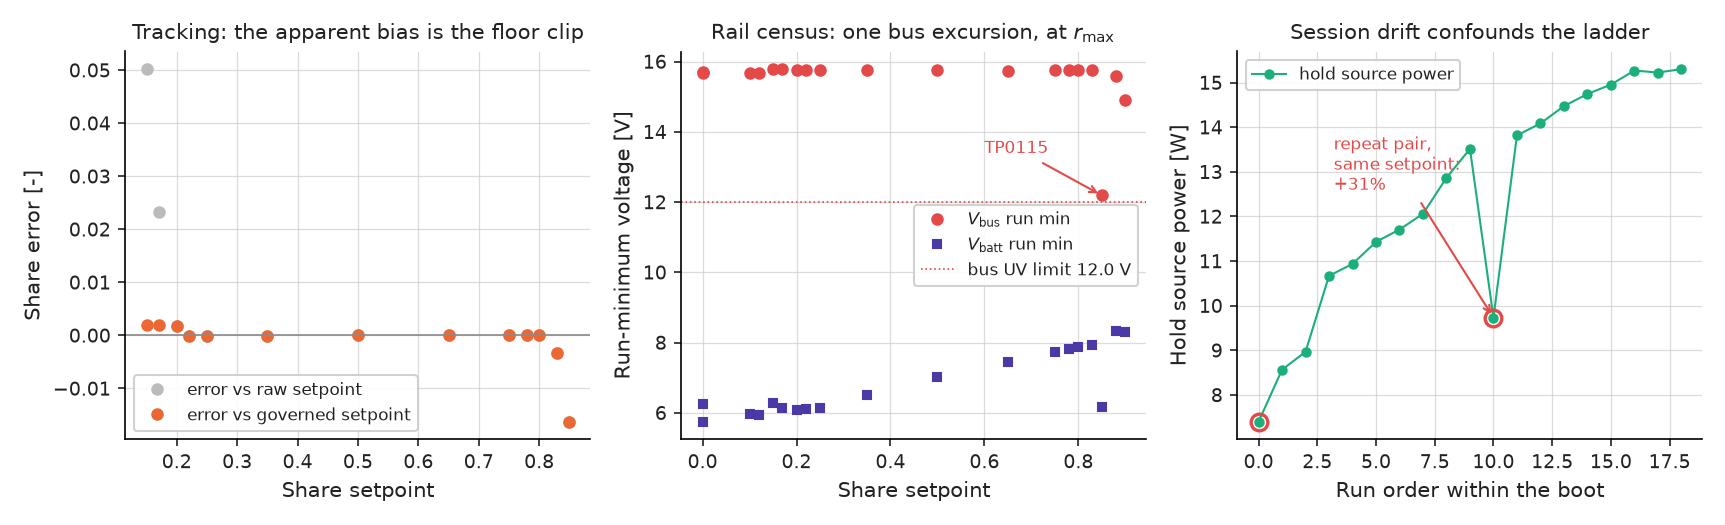
\includegraphics[width=\textwidth]{figs/fig_v6sweep_summary.png}
\caption{Firmware-v6 trapezoid ladder. Left: tracking error against the raw and
the governed setpoint; the two apparently biased points are the floor clip, not
loop error. Centre: run-minimum rails; a single bus excursion, at
$r^\ast=r_{\max}$. Right: hold source power against run order within the boot,
with the two repeat runs at $r^\ast=0$ ringed --- the ladder's monotonic
$+82\,\%$ rise is session drift, not a setpoint effect.}
\label{fig:v6summary}
\end{figure}

\subsection{The \code{W}-profile de-rating closes the firmware-v5 failure}

The R5--R7 de-rating is decisive. Table~\ref{tab:v6r6} compares the share-bound
excursion across the two firmware versions.

\begin{table}[H]
\centering
\caption{The \code{W}-profile share-bound excursion (R6), firmware~v5 versus
firmware~v6. Currents are measured channel totals inside the region.}
\label{tab:v6r6}
\begin{tabular}{llccccl}
\toprule
Run & fw & $b$ & R6 command & R6 $I_\mathrm{tot}$ med/max & R6 $V_\mathrm{bus}$ min & Outcome \\
\midrule
\code{WP0100} & v5 & 0.15 & $1.0\,I_\mathrm{max}$ & 2.01 / 2.53\,A & 15.55\,V & 28-episode dropout cycle \\
\code{WP0101} & v5 & 0.00 & $1.0\,I_\mathrm{max}$ & 2.09 / 6.12\,A & 6.13\,V & \code{ERR\_UV\_BUS} at 36\,ms \\
\code{WP0121} & v6 & 0.30 & $0.3\,I_\mathrm{max}$ & 0.14 / 0.38\,A & 15.92\,V & clean \\
\code{WP0122} & v6 & 0.20 & $0.3\,I_\mathrm{max}$ & 0.16 / 0.40\,A & 15.92\,V & clean \\
\code{WP0123} & v6 & 0.00 & $0.3\,I_\mathrm{max}$ & 0.22 / 0.50\,A & 15.87\,V & clean \\
\bottomrule
\end{tabular}
\end{table}

Measured total current in R6 falls by a factor of approximately 9.5, from
2.09\,A to 0.22\,A --- substantially more than the nominal $0.3\times$ on the
command, because the bench load is strongly nonlinear in commanded current. The
region now runs an order of magnitude below the fuel-cell source knee identified
in Section~\ref{sec:v5}. All three runs at $I_\mathrm{max}=6$\,A complete the
full 40\,s profile across the entire span of $b$, against two of seven in
firmware~v5.

The consequence is that \textbf{$b$ no longer predicts survival}. In firmware~v5
the clip bound was the whole story; here it selects only which mechanism owns
R6, and all owners are benign at 0.2\,A. Two qualifications follow. The de-rating
pushed R6 below the 0.60\,A closed-loop threshold, so closed-loop occupancy in
that region is zero: R6 no longer exercises the share controller at an extreme
command, and safety was bought by removing the interaction rather than by
surviving it. Across the whole profile, closed-loop occupancy at
$I_\mathrm{max}=6$\,A is only 17--20\,\%.

\subsection{A residual at the band edge: \code{TP0115}, $r^\ast=0.85$}
\label{sec:v6edge}

The single dropout of the ladder occurs at $r^\ast=0.85$, exactly
$r_{\max}=\code{DROOP\_R\_MAX}$, and it is the one place where firmware~v6 is
worse than firmware~v5. Table~\ref{tab:v6edge} states the comparison.

\begin{table}[H]
\centering
\caption{The band-edge setpoint on the two firmwares, same profile and same
setpoint.}
\label{tab:v6edge}
\begin{tabular}{lcc}
\toprule
Metric & firmware~v5 (\code{TP0088}) & firmware~v6 (\code{TP0115}) \\
\midrule
$V_\mathrm{bus}$ minimum & 15.75\,V & 12.19\,V \\
$V_\mathrm{batt}$ minimum & 8.01\,V & 6.17\,V \\
Total source dropout & none & 5.9\,ms \\
Fault latched & none & none \\
\bottomrule
\end{tabular}
\end{table}

Figure~\ref{fig:v6edge} resolves the event. It is not a limit cycle and not a
measurement artifact: five consecutive samples carry both channels at hard zero
while the bus decays monotonically at $0.31\,\mathrm{V\,ms^{-1}}$, after which
the battery channel reconnects at 1.81\,A and pulls its own rail from 8.35\,V to
6.17\,V. The sequence is ordered. The battery channel stops conducting one
sample after the closed-loop mode edge; the controller, seeing a measured share
of unity against its reference, drives the ratio down at the full slew limit;
24\,ms later the fuel-cell channel also drops out, leaving the bus unfed.

\begin{figure}[H]
\centering
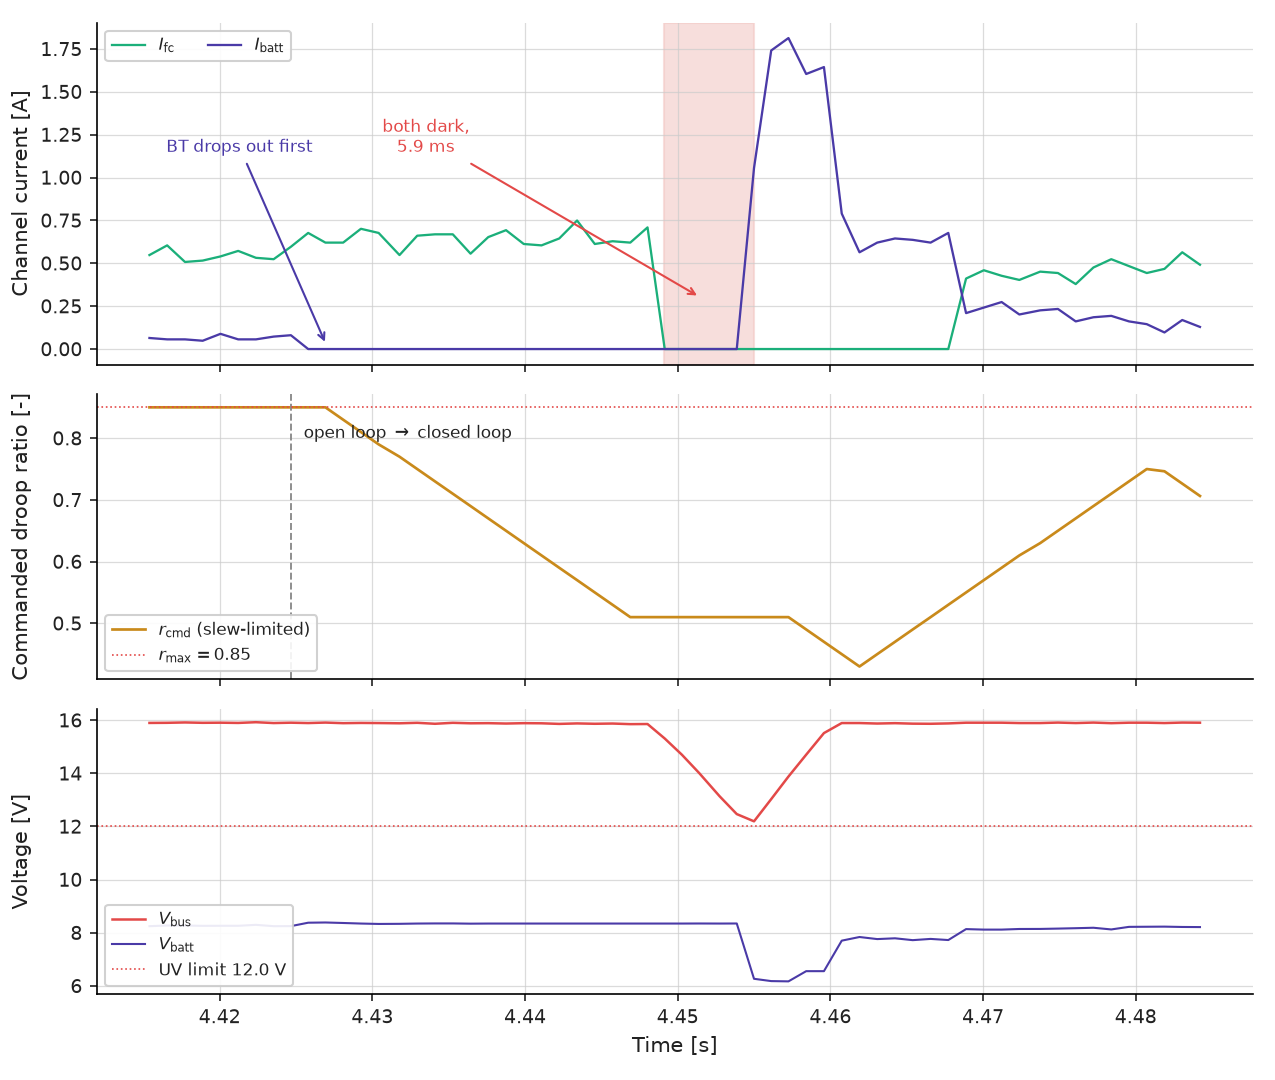
\includegraphics[width=0.92\textwidth]{figs/fig_tp0115_handover.png}
\caption{\code{TP0115}, $r^\ast=0.85$: a 5.9\,ms total source dropout at the
open-loop-to-closed-loop handover. Top: both channels dark, the battery channel
first. Centre: the commanded ratio slewing at its 0.02-per-tick limit. Bottom:
the bus decaying to 12.19\,V and the battery rail collapsing on reconnection.
Window 70\,ms of a 15\,s run.}
\label{fig:v6edge}
\end{figure}

The mechanism generalises, and the ladder contains its mirror image. Both
dropouts observed anywhere in the campaign --- \code{TP0115} at $r_{\max}$ and a
smaller fuel-cell-only event in \code{TP0105} at $r_{\min}=0.15$, which the bus
rode out at 15.89\,V --- occur at the open-loop-to-closed-loop handover, and both
at an exact band edge. Every run crosses into closed loop at the same 0.6\,A
total, where the 0.30\,A floor demands half the total current from a channel the
open-loop feedforward has been running at 61\,mA. The discriminator is monotonic
in setpoint: measured minority current in the 50\,ms before the crossing is
0.061\,A at $r^\ast=0.85$, 0.072\,A at 0.83, and 0.179\,A at 0.65.

Firmware~v6 slewed the reference \emph{rate}; the exposure is the reference
\emph{magnitude}. A swing of 0.42 in commanded share, applied at 0.6\,A total, is
enough to open both channels at once however slowly it is applied. The argument
in Section~\ref{sec:v5} against clipping the open-loop feedforward remains sound,
so the remaining lever is the crossing point itself: engaging closed-loop control
at a current where the floor's clip is less violent.

\subsection{\code{WP0124}: the failure mode moves to the source rail}

\code{WP0124} is the first run of the campaign at $I_\mathrm{max}=8$\,A. Its log
ends at $t=14.60$\,s of a 40\,s profile with no trailer record --- the signature
of an MCU stop rather than any firmware path. Two things distinguish it from
every previous truncation.

First, it died in R4, not in the share-bound excursion, and \textbf{the share
loop is a bystander}. The setpoint is 0.38, mid-band; measured share tracks it to
$\pm0.02$; both channels conduct; the bus is flat at 15.75\,V; no latch, cutoff,
deferral, or dropout occurs anywhere after $t=4.95$\,s; \code{fault\_flags} is
zero and the closed-loop mode flags are set continuously to the last record.

Second, and unlike every earlier stop, \textbf{the collapse is fully resolved on
the logged timescale}. The battery rail walks down monotonically with load ---
7.16\,V at $t=13.1$\,s, 6.55\,V at 13.9\,s, 5.99\,V at 14.5\,s, minimum
5.54\,V --- and the walk is ohmic, not dynamic. A least-squares fit over the
region gives
\begin{equation}
V_\mathrm{batt} = 8.52 - 1.35\,I_\mathrm{batt},\qquad R^2=0.982 ,
\end{equation}
against $V_\mathrm{fc} = 8.40 - 0.30\,I_\mathrm{fc}$ on the fuel-cell side.
Figure~\ref{fig:v6brownout} shows both. \textbf{The bench battery source is
approximately four times softer than the fuel-cell source}, at
$1.01$--$1.35\,\Omega$ against $0.26$--$0.30\,\Omega$. Because the Teensy is
board-powered through an LM1084 linear regulator fed from the battery rail,
drawing 1.9\,A from a $1.35\,\Omega$ source walks the microcontroller's own
supply into regulator dropout.

\begin{figure}[H]
\centering
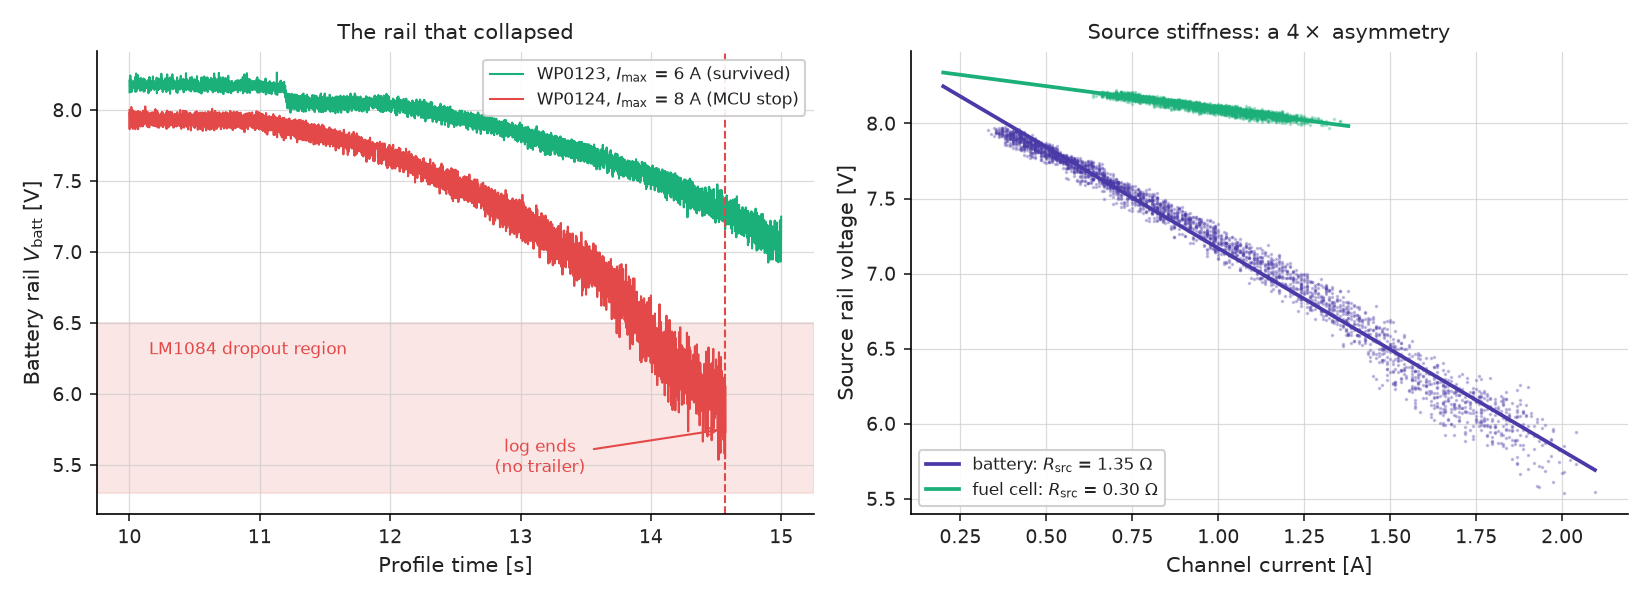
\includegraphics[width=\textwidth]{figs/fig_wp0124_brownout.png}
\caption{\code{WP0124} against its surviving twin. Left: the battery rail through
region R4; \code{WP0123} runs the same profile and the same $b$ at
$I_\mathrm{max}=6$\,A and bottoms at 6.93\,V, while \code{WP0124} at 8\,A enters
the LM1084 dropout region and the log ends. Right: source stiffness measured over
the same window.}
\label{fig:v6brownout}
\end{figure}

The comparison with \code{WP0123} is close to controlled: same profile, same
$b=0$, same firmware, differing only in $I_\mathrm{max}$. At matched profile time
the 8\,A run draws 1.83 times the battery current and its rail sits 1.28\,V
lower. The causal chain is therefore $I_\mathrm{max} \rightarrow I_\mathrm{batt}
\rightarrow V_\mathrm{batt} \rightarrow$ logic rail, with the share loop
uninvolved --- structurally different from the firmware-v5 stops, which were
share-mediated fuel-cell source-knee runaways.

This finding subsumes rather than contradicts the oscilloscope evidence of
Section~\ref{sec:v5}: the direct-current operating point had already walked into
the region where the sub-millisecond dip resolved in capture~14 lands far below
the dropout threshold. It remains inference. Neither the regulator output nor
the Teensy 3.3\,V rail is logged or was probed through this stop.

\subsection{Why no battery-rail undervoltage threshold is proposed}
\label{sec:v6nothresh}

The obvious remedy is the battery-side counterpart of the new fuel-cell
undervoltage fault. The data does not support one on this bench, and the reason
is itself informative.

Replaying the firmware-v6 leaky-dwell filter against the logged battery rail of
every run in the campaign gives Figure~\ref{fig:v6thresh}. Healthy trapezoid runs
in which the battery is the sole source sag as low as 5.75\,V and complete
without incident, while \code{WP0124} died at 5.54\,V. A trip at 6.8\,V or 6.5\,V
latches six healthy runs; a trip at 6.0\,V still latches \code{TP0112}; a trip at
5.7\,V catches nothing at all, including the truncation.

\begin{figure}[H]
\centering
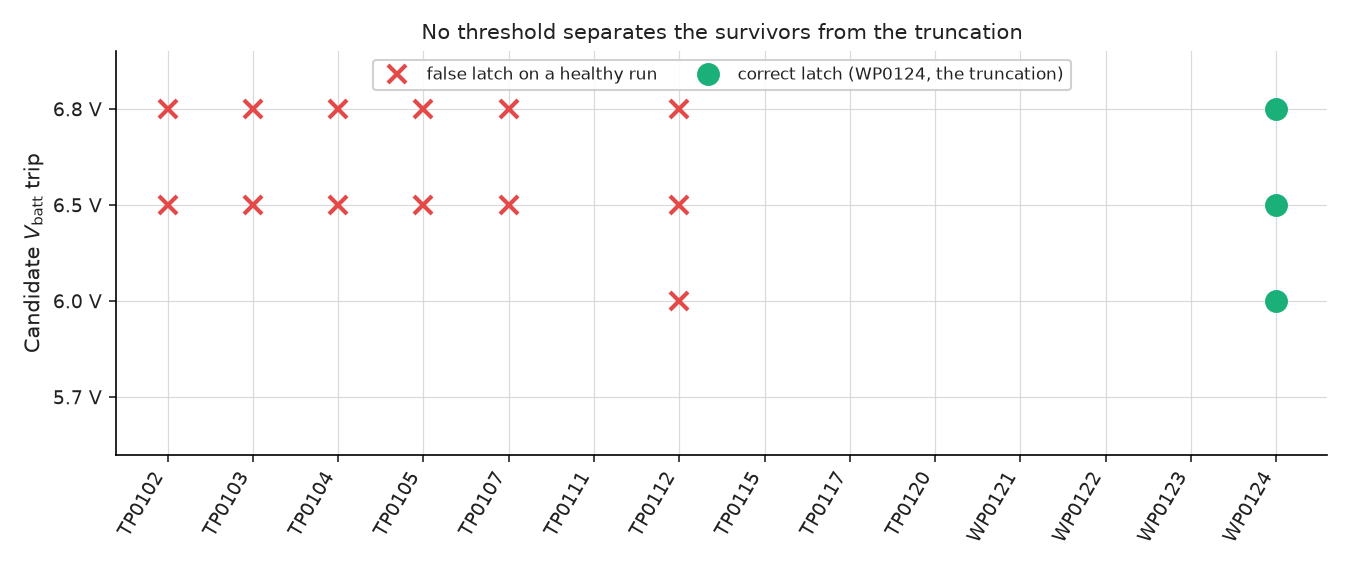
\includegraphics[width=\textwidth]{figs/fig_vbatt_threshold.png}
\caption{The firmware-v6 leaky-dwell filter replayed against the logged battery
rail at four candidate trip voltages. No row separates the truncation from the
healthy runs.}
\label{fig:v6thresh}
\end{figure}

A separation of roughly 0.2\,V across a hard survive-or-die boundary is the
signature of a \emph{cliff} --- the regulator dropout knee --- rather than of a
gradual margin. It follows that the logged direct-current level under-determines
the outcome, and that the real discriminator is the sub-millisecond ripple depth
riding on it, which is precisely what capture~14 resolves and what an 870\,Hz log
cannot see. A threshold fitted to this data would therefore encode bench
conditions rather than the failure mechanism. The blocking measurement is
unchanged from Section~\ref{sec:v5}: the LM1084 input and output, probed together
through a truncation.

\subsection{Two limits on what this campaign can conclude}

\textbf{The headline mechanism of firmware~v6 remains unvalidated on the bench.}
The deferral branch of the load-aware handoff guard did not engage in any of the
23 runs. Every setpoint latch in the campaign handed off 0.06--0.24\,A, far below
the 0.50\,A threshold, so only the permitting branch executed.
$I_\mathrm{handoff}^{\max}$ is still bracketed only between an observed-clean
0\,A and an observed-fatal 1.3\,A. The de-rating has made this harder to test,
not easier: it removed the only condition that previously produced a loaded
out-of-band setpoint. The new fuel-cell undervoltage fault is likewise untested
--- correct and silent, but with the rail never closer than 1.67\,V to its trip.

\textbf{Session drift confounds the ladder.} The two repeat runs at $r^\ast=0$,
914\,s apart within the same boot, differ by $+31\,\%$ in hold source power at a
fixed setpoint, and hold power rises monotonically by $82\,\%$ across the ladder
(Figure~\ref{fig:v6summary}, right). Because setpoint was swept monotonically
with run order, the setpoint effect and the drift are not separable in this
campaign. The interleaving recommended after the firmware-v2 round was not
applied. Since the total current sets the governor's own clip threshold, the
per-setpoint operating points are not directly comparable across the ladder.

\section{Conclusions and recommended actions}
\label{sec:conclusions}

From the discovery sweep (firmware~0):

\begin{enumerate}
\item \textbf{The share controller is validated across the full setpoint span at
steady load}: unbiased ($<10^{-3}$) at all seven setpoints, $\sigma\approx0.01$ at
interior points, no saturation for $r^\ast\in[0.15,0.7]$.
\item \textbf{A 17--18.5\,Hz minority-channel dropout limit cycle exists at
asymmetric setpoints under low total current}, severe at $r^\ast=0.3$ (bus to
6.5\,V, 3.6\,A spikes) and mild at $r^\ast=0.85$. Capture~12 confirms the events are
total source-feed dropouts (motor switch conducting, whole bus decaying together);
droop-commanded blocking vs.\ source-switch SCP remains open but no longer gates the
fix.
\end{enumerate}

From the validation sweep (firmware~v3):

\begin{enumerate}
\setcounter{enumi}{2}
\item \textbf{The mitigation set works where it applies.} All 20 in-band runs from
$r^\ast=0.18$ to 0.85 --- the two original failure points included --- are free of
dropout events, with unbiased tracking and a flat bus; the moving-setpoint run
\code{WP0040} tracks the governed command with residuals $\leq2\times10^{-3}$
through simultaneous setpoint and load steps. The governor floor is directly
observable holding the minority channel at 0.20\,A~$\pm$5\,\%.
\item \textbf{$I_\mathrm{min}=0.20$\,A sits on the failure boundary, not above
it.} \code{TP0016} ignites at the exact governor release instant; the empirical
conduction floor lies in $(0.245, 0.29)$\,A. Raise
\code{SHARE\_MINORITY\_I\_MIN\_A} to $\approx$0.30\,A. Independently, the band-edge
setpoint parks the actuator on the \code{DROOP\_R\_MIN} rail inside the cutoff
hysteresis; treat the usable in-band span as $\approx[0.18, 0.82]$.
\item \textbf{Close the governor/cutoff structural gap.} The governor bypass tests
the \emph{setpoint} while the cutoff tests the \emph{controller output}; setpoints
in $\approx(0.85, 0.88]$ (mirror $\approx[0.12, 0.15)$) engage neither and run the
original cycle unmitigated (\code{TP0037}). Either extend the governor to the full
span and let the cutoff take over only once it actually latches, or gate the bypass
on the cutoff state (\code{shareIsoFC}/\code{shareIsoBT}) rather than on the
setpoint. The near-band cutoff \emph{hunting} at $r^\ast=0.12$ (19.8\,Hz
switch duty-cycling) additionally argues for latching the cutoff while the
setpoint remains out-of-band, releasing on setpoint change rather than on the
ratio's re-entry hysteresis.
\item \textbf{Arm a bus-undervoltage fault on the bench.} Both \code{TP0016} and
\code{WP0039} put the bus below 9\,V repeatedly with \code{fault\_flags}~$=0$;
\code{WP0039} ended in an uncommanded MCU brownout. A persistence-filtered UV check
(mirroring the existing OV filter) would have latched both runs into State~99 long
before the ratchet deepened.
\item \textbf{Scope-armed follow-ups}: re-enter the \code{WP0039} condition to
test the unfreeze-slew-traverse trigger correlation and identify why the motor
accepted no load for 11.8\,s; probe a boost output alongside VBUS during a
\code{TP0016} hold to close the droop-blocking vs.\ SCP discrimination; check the
$\approx$14\,\% control-tick slowdown against the firmware timing.
\end{enumerate}

Items~4--6 were implemented as firmware~v4. From the second validation sweep
(firmware~v4):

\begin{enumerate}
\setcounter{enumi}{7}
\item \textbf{The setpoint-latched cutoff and the raised floor close every
firmware~v3 failure point.} All out-of-band setpoints latch once with zero
switch cycling (0.12: 179 cycles to zero; 0.88--0.90: continuous limit cycle to
a static latch), and the band edge 0.15 holds its commanded minority at exactly
0.3000\,A with a flat bus. The governed band tracks with bias below $10^{-3}$
and the \code{W} profiles reproduce the governor law to $\leq 2\times10^{-3}$.
\item \textbf{Redesign the governor's low-current fallback.} The
collapse-to-0.5 branch commands 0.05--0.25\,A per channel across
$I_\mathrm{tot} \in [0.075, 0.60]$\,A --- below the floor it exists to enforce ---
and ignited a bus-collapsing source-commutation relay cycle in six runs at
$r^\ast \geq 0.67$ (Section~\ref{sec:relay}). The fallback should command an
\emph{achievable} split at low current: hold the measured share (freeze the
loop, as the setpoint latch already does out-of-band) or bias toward the natural
topology, rather than force 0.5. Why firmware~v3 survived the identical
conditions is unconfirmed; the floor increase acting through the escape window
is the leading candidate.
\item \textbf{The constant-current floor law is wrong.} At region R6 the
firmware~v4 clean/cycling bracket of $(0.381, 0.399)$\,A contradicts the
firmware~v3 bracket of $(0.245, 0.29)$\,A; either the floor scales with total
current or the true limit is a minority fraction of $\approx$0.22--0.25. A
two-axis sweep ($I_\mathrm{max}$ at fixed setpoint, setpoint at fixed
$I_\mathrm{max}$) separates the two readings and sets the corrected law.
\item \textbf{Extend fault coverage upstream and retune the UV filter.} The UV
fault latched all six relay events but tolerated 1.0--1.3\,s of 7--8\,V
excursions first (the 9\,ms-under/51\,ms-over duty evades the 10\,ms window and
5\,ms gap guard); a leaky-integrator dwell or a $\gtrsim$60\,ms gap guard
latches within a few cycles. More consequentially, two MCU brownouts occurred
with the bus in regulation at 15.7\,V: the source rail feeding the logic
regulator is unobserved. Log \code{BT\_VOLTAGE}, consider a source-rail
undervoltage fault, and scope \code{VBT}/LM1084 across the R6$\to$R7 setpoint
step before further $b \leq 0.22$ runs.
\end{enumerate}

Items~9, 11 (in part), and~12 were implemented as firmware~v5. From the third
validation sweep (firmware~v5):

\begin{enumerate}
\setcounter{enumi}{11}
\item \textbf{The open-loop fallback closes the relay cycle.} The four
firmware~v4 relay setpoints run clean --- zero exclusive conduction, no
14--24\,Hz signature, bus flat at 15.7\,V --- and the feedforward, hold-freeze,
and mode hysteresis are each directly observable in the logs with zero chatter.
One tidy-up remains: apply the governor clip to the feedforward path so the
handover at 0.60\,A does not step the effective setpoint discontinuously.
\item \textbf{The \code{W}-profile R6 excursion is a test-design hazard and a
finding in one.} It is the only region combining peak load with an extreme
share command, and it generated all five failures. Do not run \code{W}/\code{Y}
profiles with $b < 0.30$ until the region drops its motor axis; record $b$ and
$I_\mathrm{max}$ in the log header. Separately, the $b=0$ case shows the
setpoint-latched cutoff acting as an under-load channel cut that collapses the
surviving source in 40\,ms --- the latch needs a load-aware guard (defer the cut,
or ramp it, when the surviving channel cannot carry the measured total).
\item \textbf{The floor law is structurally wrong, not miscalibrated.} The
battery channel drops out at commanded minority currents of 0.55--1.04\,A ---
two to three times the 0.30\,A floor --- while the fuel-cell channel holds
0.63\,A as minority with no dropout, and 27\,mV of bus voltage separates a
28-dropout operating point from a stable one. The boundary is a
bus-versus-reference margin, one-sided toward the battery channel; replace the
current constant with a reference-referred guard and run the two-axis sweep per
channel direction.
\item \textbf{The dwell filter is validated; the missing fault is upstream.}
Both latching runs latch within $\approx$20\,ms of first excursion (firmware~v4:
1.0--1.3\,s), with no spurious latch in 28 runs. The three MCU stops beat the
filter from the source side: the fuel-cell rail sat below 5\,V while the bus
still read 15.7\,V, and the battery rail read 7.9--8.4\,V at every truncation
instant --- so a source-rail undervoltage fault (dwell-filtered, on the logged
rails) is the highest-value protection now missing. Oscilloscope capture~14
resolves a sub-millisecond battery-rail dip to $\approx$4--5\,V, coincident
with a battery-current spike as the collapsing node reaches the battery-rail
level --- the leading MCU-stop candidate, below the LM1084 dropout and
invisible to the log --- pending confirmation by a capture on the LM1084
input and output through a truncation event.
\end{enumerate}

Items~13--15 were implemented as firmware~v6. From the fourth validation sweep
(firmware~v6):

\begin{enumerate}
\setcounter{enumi}{15}
\item \textbf{The profile de-rating and the reference slew are validated.} The
share-bound excursion carries 0.22\,A instead of 2.09\,A, an order of magnitude
below the source knee; all three combined-profile runs at $I_\mathrm{max}=6$\,A
complete across the full span of $b$, which no longer predicts survival. The
commanded ratio never moves faster than its 0.02-per-tick limit in any of the 23
runs, and the governor floor is exact to $10^{-3}$. Note the cost: the de-rated
region now runs entirely below the closed-loop threshold, so it no longer tests
the share controller at an extreme command. If that case still needs
characterising it needs a separate, deliberately bounded region.
\item \textbf{Move the closed-loop engagement point, not the reference rate.} The
one dropout of the ladder --- 5.9\,ms with both channels dark and the bus at
12.19\,V --- occurs at the open-loop-to-closed-loop handover at the exact upper
band edge, and its mirror appears at the lower edge. The floor demands half the
total current from a channel carrying 61\,mA at the crossing; a 0.42 swing in
commanded share at 0.6\,A total opens both channels however slowly it is applied.
Raising \code{SHARE\_GOV\_OL\_HYST\_A} so closed-loop control engages where the
clip is less violent addresses the magnitude; the firmware~v6 slew addressed only
the rate.
\item \textbf{Stiffen the battery source or power the logic independently.} The
bench battery source measures $1.01$--$1.35\,\Omega$ against $0.26$--$0.30\,\Omega$
on the fuel-cell side, and the sole truncation of the campaign is an ohmic
collapse of that rail into the logic regulator's dropout region with the share
loop tracking to $\pm0.02$ and the bus in regulation. On this bench
$I_\mathrm{max}$ is bounded by the logic rail rather than by anything in the
control law, and the bound was reached at 8\,A.
\item \textbf{Do not fit a battery-rail undervoltage threshold to this data.}
Replaying the dwell filter across the campaign, healthy runs sag to 5.75\,V and
complete while the truncation died at 5.54\,V; every trip that catches the
truncation also latches healthy runs. A 0.2\,V separation across a survive-or-die
boundary indicates a regulator dropout cliff, so the logged operating point
under-determines the outcome and the discriminator is the sub-millisecond ripple
depth. The blocking measurement is unchanged: LM1084 input and output probed
together through a truncation.
\item \textbf{The load-aware handoff guard is still unvalidated, and the
de-rating made it harder to test.} Its deferral branch did not engage in any of
the 23 runs; every latch handed off 0.06--0.24\,A against a 0.50\,A threshold, so
only the permitting branch ran. $I_\mathrm{handoff}^{\max}$ remains bracketed
between an observed-clean 0\,A and an observed-fatal 1.3\,A. Exercising it now
requires a deliberately constructed loaded out-of-band setpoint, since the
de-rated excursion no longer produces one. The new fuel-cell undervoltage fault
is likewise correct but untested, its rail never closer than 1.67\,V to trip.
\item \textbf{Interleave the setpoint order.} The two repeat runs at $r^\ast=0$
differ by $+31\,\%$ in hold source power within one boot, and hold power rises
monotonically by $82\,\%$ across the ladder. Setpoint was swept monotonically
with run order, so the setpoint effect and the session drift are not separable in
this campaign --- and since total current sets the governor's own clip threshold,
the per-setpoint operating points are not comparable across it. This hygiene was
recommended after the firmware-v2 round and has still not been applied.
\end{enumerate}

\end{document}
